\documentclass[]{msu-thesis}
\usepackage{lmodern}
\usepackage{amssymb,amsmath}
\usepackage{ifxetex,ifluatex}
\usepackage{fixltx2e} % provides \textsubscript
\ifnum 0\ifxetex 1\fi\ifluatex 1\fi=0 % if pdftex
  \usepackage[T1]{fontenc}
  \usepackage[utf8]{inputenc}
\else % if luatex or xelatex
  \ifxetex
    \usepackage{mathspec}
  \else
    \usepackage{fontspec}
  \fi
  \defaultfontfeatures{Ligatures=TeX,Scale=MatchLowercase}
\fi
% use upquote if available, for straight quotes in verbatim environments
\IfFileExists{upquote.sty}{\usepackage{upquote}}{}
% use microtype if available
\IfFileExists{microtype.sty}{%
\usepackage{microtype}
\UseMicrotypeSet[protrusion]{basicmath} % disable protrusion for tt fonts
}{}
\usepackage[margin=1in]{geometry}
\usepackage{hyperref}
\hypersetup{unicode=true,
            pdftitle={Understanding Work With Data in Summer STEM Programs Through An Experience Sampling Method Approach},
            pdfauthor={Joshua M. Rosenberg},
            pdfborder={0 0 0},
            breaklinks=true}
\urlstyle{same}  % don't use monospace font for urls
\usepackage{natbib}
\bibliographystyle{apalike}
\usepackage{longtable,booktabs}
\usepackage{graphicx,grffile}
\makeatletter
\def\maxwidth{\ifdim\Gin@nat@width>\linewidth\linewidth\else\Gin@nat@width\fi}
\def\maxheight{\ifdim\Gin@nat@height>\textheight\textheight\else\Gin@nat@height\fi}
\makeatother
% Scale images if necessary, so that they will not overflow the page
% margins by default, and it is still possible to overwrite the defaults
% using explicit options in \includegraphics[width, height, ...]{}
\setkeys{Gin}{width=\maxwidth,height=\maxheight,keepaspectratio}
\IfFileExists{parskip.sty}{%
\usepackage{parskip}
}{% else
\setlength{\parindent}{0pt}
\setlength{\parskip}{6pt plus 2pt minus 1pt}
}
\setlength{\emergencystretch}{3em}  % prevent overfull lines
\providecommand{\tightlist}{%
  \setlength{\itemsep}{0pt}\setlength{\parskip}{0pt}}
\setcounter{secnumdepth}{5}
% Redefines (sub)paragraphs to behave more like sections
\ifx\paragraph\undefined\else
\let\oldparagraph\paragraph
\renewcommand{\paragraph}[1]{\oldparagraph{#1}\mbox{}}
\fi
\ifx\subparagraph\undefined\else
\let\oldsubparagraph\subparagraph
\renewcommand{\subparagraph}[1]{\oldsubparagraph{#1}\mbox{}}
\fi

%%% Use protect on footnotes to avoid problems with footnotes in titles
\let\rmarkdownfootnote\footnote%
\def\footnote{\protect\rmarkdownfootnote}

%%% Change title format to be more compact
\usepackage{titling}

% Create subtitle command for use in maketitle
\newcommand{\subtitle}[1]{
  \posttitle{
    \begin{center}\large#1\end{center}
    }
}

%\setlength{\droptitle}{-2em}
%  \title{Understanding Work With Data in Summer STEM Programs Through An Experience Sampling Method Approach}
%  \pretitle{\vspace{\droptitle}\centering\huge}
%  \posttitle{\par}
%  \author{Joshua M. Rosenberg}
%  \preauthor{\centering\large\emph}
%  \postauthor{\par}
%  \predate{\centering\large\emph}
%  \postdate{\par}
%  \date{2017-11-24}
%

\frontmatter
%\pagenumbering{Roman}
\newpage

\newpage

\pagebreak

\pagebreak


\usepackage{booktabs}
\usepackage{amsthm}
\makeatletter
\def\thm@space@setup{%
  \thm@preskip=8pt plus 2pt minus 4pt
  \thm@postskip=\thm@preskip
}
\makeatother
\setlength{\parindent}{4em}
\setlength{\parskip}{0em}

\title{Understanding Work With Data in Summer STEM Programs Through An Experience Sampling Method Approach}
\author{Joshua M. Rosenberg}
\fieldofstudy{Educational Psychology and Educational Technology}
\dedication{This dissertation is dedicated to Katie and to Jonah, who (mostly) happily slept through most of its writing.}
\date{2018}

%%%%%% MSU-THESIS stuff
% \usepackage[T1]{fontenc}
% \usepackage{newtxtext,newtxmath} % If they want Times we’ll give them Times
% \usepackage{amsmath}
% %
% \usepackage[]{natbib}
% \bibliographystyle{unified}
%
%
% % If you need newlines in your title, you must use \protect\\
% \title{Understanding Work With Data in Summer STEM Programs Through An Experience Sampling Method Approach}
% \author{Joshua M. Rosenberg}
% \fieldofstudy{Educational Psychology and Educational Technology}
% \dedication{This dissertation is dedicated to Katie and to Jonah, who (mostly) happily slept through most of its writing.}
% \date{2018}
% \usepackage{listings}
% \lstset{language=TeX,basicstyle={\ttfamily}}
% \usepackage{lipsum}
% \usepackage{xcolor}
% \usepackage{gb4e}
%
% %\usepackage[bookmarksopenlevel=2,bookmarks=true]{hyperref} % not needed but here for testing
%
% \counterwithin{exx}{chapter}
% \singlegloss
%
% % Uncomment the next line for single spaced examples with gb4e
% %\patchcommand{\exe}{\SingleSpacing}{}
%
% % This code is an example of how to set up a new list of
% \newlistof{listoflistings}{lol}{List of Listings}
% \newfloat[chapter]{listing}{lol}{Listing}
% \newlistentry{listing}{lol}{0}
% \renewcommand*{\cftlistingname}{Listing\space}
% \renewcommand*{\cftlistingaftersnum}{\msucaptiondelim}
\usepackage{booktabs}
\usepackage{longtable}
\usepackage{array}
\usepackage{multirow}
\usepackage[table]{xcolor}
\usepackage{wrapfig}
\usepackage{float}
\usepackage{colortbl}
\usepackage{pdflscape}
\usepackage{tabu}
\usepackage{threeparttable}

\usepackage{amsthm}
\newtheorem{theorem}{Theorem}[section]
\newtheorem{lemma}{Lemma}[section]
\theoremstyle{definition}
\newtheorem{definition}{Definition}[section]
\newtheorem{corollary}{Corollary}[section]
\newtheorem{proposition}{Proposition}[section]
\theoremstyle{definition}
\newtheorem{example}{Example}[section]
\theoremstyle{definition}
\newtheorem{exercise}{Exercise}[section]
\theoremstyle{remark}
\newtheorem*{remark}{Remark}
\newtheorem*{solution}{Solution}
\begin{document}
%\maketitle

\maketitlepage
% Next make the abstract
\begin{abstract}
% Your abstract goes here.  Master's 1 page max. PhD 2 page max.

Data-rich activities provide an opportunity to develop core competencies in both science and mathematics identified in curricular standards. Perhaps even more importantly work with data puts learners in the position to use data to ask and answer questions, a potentially empowering capability. Research on work with data has focused on cognitive outcomes and the development of specific practices at the student and classroom levels, and yet, little research has considered learners’ engagement. The present study explores learners engagement in work with data in the context of summer STEM programs. The aspects of work with data that are the focus of this study are: asking questions, observing phenomena, constructing measures and generating data, data modeling, and interpreting findings. Data from measures of learners' engagement was collected through the Experience Sampling Method (ESM) that involves asking learners at random intervals to answer short questions about their engagement to discover profiles of learners' engagement.

Data was collected from nine summer STEM programs over four weeks in the Northeastern United States. 203 learners reported 2,970 responses via short ESM surveys of how engaged they were (cognitively, behaviorally, and affectively, assessed through separate items) and of their perceptions of themselves (their competence) and the activity (its challenge).  These data were used to examine five specific research questions: 1) What is the frequency and nature of opportunities for youth to engage in each of the five aspects of work with data in summer STEM programs? 2) What profiles of engagement emerge from data collected via ESM in the programs? 3) What are sources of variability for the profiles of engagement? 4) How do the five aspects of work with data relate to profiles of engagement? 5) How do youth characteristics relate to profiles of engagement?

Findings show that aspects of work with data were fairly common overall, but that work with data was enacted out in varying ways, including some that were possibly highly engaging. Six profiles of youth engagement were identified, representing distinct configurations of the five indicators of engagement. Substantial variability in the profiles was present at the youth level, with less explained by the program youth were in or the nature of the particular instructional episode present at the times when youth were signaled. Relations between the profiles of engagement and each of the aspects of work with data were somewhat small: Notable exceptions were the generating data and data modeling were significantly associated with full engagement. Youth with higher pre-program interest in STEM were more likely to be engaged and competent but not challenged, though other youth characteristics were not highly related to the profiles.

I discuss key findings as regards work with data in summer STEM programs and other informal learning environments, the nature of youths' engagement, and what factors can predict engagement. The design and goals of summer STEM programs, which are not (necessarily) focused on activities related to work with data, as well as other limitations including the measures for work with data used and the analytic approach, are identified and described. The role of generating data and modeling data as well as attention to the specifics of how work with data are enacted are presented as implications for practice. I highlight aspects of the findings and the implications for practice with respect to work with data in general and to engagement in informal learning environments, such as summer STEM programs, in both cases with an emphasis on how work with data can serve as a promising context for learning in STEM subject areas.

\end{abstract}

% Force a newpage
\clearpage
% Make the copyright page. The Graduate School ridiculously prohibits you
% from having a copyright page unless you pay ProQuest to register the copyright.
% This should be illegal, but I didn't make up the rule.

\makecopyrightpage

% If you have a dedication page, uncomment the next command to print the dedication page
%
\makededicationpage
%
\clearpage

% Your Acknowledgements are formatted like a chapter, but with no number
\chapter*{Acknowledgements}
\DoubleSpacing % Acknowledgements should be double spaced
I would like to acknowledge my advisor and dissertation co-director Matthew Koehler and my dissertation co-director Jennifer Schmidt. I would also like to thank Lisa Linnenbrink-Garcia and Christina Schwarz. Thank you to my mentors and peers in the EPET program at MSU. Thank you to collaborators Lee Shumow and Neil Naftzger for their work on the STEM Interest and Engagement project (National Science Foundation DRL-1421198), of which this project is a secondary analysis. Thank you to participating youth activity leaders and youth.

Code for all of th analyses as well as all of the files used to generate this document are hosted in a publicly-accessible repository here: https://github.com/jrosen48/dissertation

Please note that this material is based upon work supported by the National Science Foundation under Grant No. 1421198). Any opinions, findings, conclusions, or recommendations expressed in this material are those of the authors and do not reflect the views of the National Science Foundation.

Understanding Work With Data in Summer STEM Programs Through An Experience Sampling Method Approach is licensed under a Creative Commons Attribution-ShareAlike 4.0 International License.
\clearpage

% We need to turn single spacing back on for the contents/figures/tables lists
\SingleSpacing
\tableofcontents* % table of contents will not be listed in the TOC
\clearpage
\listoftables % comment this out if you have no tables
\clearpage
\listoffigures % comment this out if you have no figures
\mainmatter
% If you have a list of abbreviations/symbols it would go here preceded by a \clearpage
% See the class documentation and the Memoir manual for how to create other lists
%

\chapter{Introduction}\label{intro}

\DoubleSpacing

Socializing, working, and even teaching and learning are increasingly
impacted by data. These sources of data are created by us, for us, and
about us. Work with data in education may be a valuable context for
teaching and learning because it reverses the role that teachers and
especially learners commonly find themselves in, namely, as the targets
of the work of data analysts and policymakers. In particular, work with
data empowers learners to--themselves--use data to ask and answer
questions. In turn, work with data promotes learners to create new
knowledge, too, in addition to learning about the key ideas and
practices of a subject matter domain.

Work with data includes broad processes of collecting, creating,
modeling data, and even asking questions that can be answered with data.
This work, then, is more than just crunching numbers. It is also more
than interpreting a figure created by someone else. Instead, work with
data is about making sense of phenomena in the world--or solving
problems in the world. This focus on phenomena is particularly relevant
to those designing and enacting learning opportunities focused on work
with data (Lee \& Wilkerson, 2018; Singer, Hilton, \& Schweingruber,
2006; Wild \& Pfannkuch, 1999).

Despite not being very prevalent, aspects of work with data cut across
STEM (science, technology and computer science, engineering, and
mathematics) domains: Aspects of work with data are recognized as core
competencies across recent curricular documents. They are found, for
example, in the \emph{Next Generation Science Standards} (NGSS Lead
States, 2013) and the \emph{Common Core State Standards} (in
mathematics; National Governors Association Center for Best Practices,
Council of Chief State School Officers, 2010). Both of these standards
highlight the role of authentic work with data. Thus, work with data can
be empowering not only because it positions learners as creators of new
knowledge about the world, but also because it can support the
development of capabilities that learners can use across subject areas.
These capabilities may be particularly useful in STEM domains because
advanced coursework in these domains often involves demanding and
abstract work with data, work that may be more accessible to more
learners when they encounter it earlier in their education.

Past research on work with data has mostly been set in mathematics
contexts and has focused on mathematical practices, like generating
measures of phenomena and creating data models (English, 2012; Lehrer \&
Romberg, 1996; Lesh, Middleton, Caylor, \& Gupta, 2008). It has often
focused on specific cognitive outcomes (e.g., Gelman \& Markman, 1987),
strategies to support work with data (Petrosino, Lehrer, \& Schauble,
2003), and some opportunities and challenges facing both teachers and
learners when working with data (e.g., Konold \& Pollatsek, 2002). There
has been some research about work with data in science settings (Lee \&
Wilkerson, in press; National Research Council, 2012), though this work
varies greatly concerning the nature of work with data (McNeill \&
Berland, 2017). Findings from this past research broadly suggest that
engaging in work with data is powerful concerning learning both about
and how to do mathematics and science. Lehrer and Schauble (2015),
summarizing past research on the use of mathematical practices in
science contexts, note that work with data ``has an exceptionally high
payoff in terms of students' scientific reasoning'' (Lehrer \& Schauble,
2015, p.~696).

To date, past research shows that using a framework from contemporary
engagement theory to characterize students' experiences has been
informative both in research and to practicing educators. Work with data
might be engaging to youth because past research has shown hands-on,
laboratory work, to which work with data is similar---to be (Schmidt,
Rosenberg, \& Beymer, 2018). In addition, work with data is demanding
and requires sustained effort and focus (Lehrer \& Schauble, 2015;
National Research Council, 2015), and past work has shown that when
learners are more challenged (and competent), they are more likely to be
engaged (Schneider et al., 2016; Shernoff et al., 2016). Knowing more
about how youth engage in work with data is valuable as engagement is a
meaningful outcome for STEM learners in its own right (Sinatra, Heddy,
\& Lombardi, 2015). It may also be an antecedent of changes in other
outcomes, such as their well-being, achievement, and the pursuit of an
area of study or career (Wang, Chow, Hofkens, \& Salmela-Aro, 2015; Wang
\& Eccles, 2012). However, research has not examined engagement in work
with data. Because engaging in work with data seems to be so potentially
beneficial to learners, better understanding the nature of work with
data and learners' engagement in such practices is needed.

The purpose of this study, then, is to examine youth engagement in a
variety of learning activities that involve work with data. I explore
youths' engagement in the context of outside-of-school STEM enrichment
programs carried out during the summer, and I consider work with data
through the lens of specific aspects identified from past research, such
as asking questions and generating and modeling data. Such settings (in
outside-of-school programs) are an especially useful context for
exploring work with data because they can be designed around youths'
interests (Lauer, Akiba, Wilkerson, Apthorp, Snow, \& Martin-Glenn,
2006). One promise of work with data in outside-of-school settings is
that data can be inherently interesting to learners and can be used as a
context for learning about the world, allowing youth to ask and answer
personally and socially meaningful questions, whereas many
outside-of-school programs are focused around commercial aims, such as
developing mobile device applications. Knowing more about how youth
engage can also provide a foundation for subsequent work to explore how
particular curricula and engaging experiences for youth spark their
interest in work with data, including hobbies and occupations related to
data science, but also in STEM domains in general.

\chapter{Literature Review}\label{literature-review}

The framework for this study is informed by work on STEM-related
learning practices, student engagement, and approaches to analyzing
complex psychological constructs, like engagement. In this review of the
literature, I define work with data as a key practice, or
learning-related activity, across STEM domains. I also define and
justify a multi-dimensional framework for understanding engagement, and
then review an approach to analyzing data that is ideal for capturing
this multidimensionality.

\section{Defining Work with Data}\label{defining-work-with-data}

Some scholars have focused on a few key pieces of data analysis,
connected through the use of ``data to solve real problems and to answer
authentic questions'' (Hancock et al., 1992, p.~337). This focus on
solving real problems or answering authentic questions--rather than
being taught and learned as isolated skills--is an essential part of
work with data having the most educational benefits to learners
(National Research Council, 2012; see Lehrer and Schauble {[}2012{]}
Windschitl, Thompson, \& Braaten {[}2018{]} for excellent, practice,
in-depth examples of work with data being used as part of instructional
approaches). This approach has primarily been used by mathematics
educators, as reflected in its role in statistics curriculum standards
(Franklin et al., 2007). In science settings, where answering questions
about phenomena serve as the focus of activities, it shares features of
the process of engaging in scientific and engineering practices but has
been less often studied.

Work with data has been conceived in different ways (i.e., Hancock et
al., 1992; Lehrer \& Romberg, 1996; Wild \& Pfannkuch, 1999). For
instance, Wild and Pfannkuch (1999) consider the process in terms of
identifying a problem, generating a measurement system and sampling
plan, collecting and cleaning the data, exploring the data and carrying
out planned analyses, and interpreting the findings from the analysis.
Such a process is common in STEM content areas, particularly across
statistics education research and is instantiated in standards for
curricula: Franklin et al.'s guidelines for the American Statistical
Association focus on the Framework for statistical problem solving:
formulating questions, collecting data, analyzing data, and interpreting
results (2007). The goals of this framework and its components are
similar to Hancock et al.'s (1992) description of data modeling, the
process of ``using data to solve real problems and to answer authentic
questions'' (p.~337). Hancock et al. (1992) focus in on two goals, data
creation and analysis, arguing that the former (data creation) is ``the
neglected counterpart of data analysis'' (p.~339). Scholars have
subsequently expanded Hancock et al.'s definition of data modeling to
include six components: asking questions, generating measures,
collecting data, structuring data, visualizing data, and making
inferences in light of variability (see Lehrer \& Schauble, 2004, for
use of this conceptualization of data modeling applied to the task of
understanding how plants grow). The last of these components is crucial
across all of the visions of data modeling reviewed here and
distinguishes these processes from other aspects of data analysis:
Accounting for variability (or uncertainty) is central to solving
real-world problems with data and the process of data modeling.

Because there is not an agreed-upon definition of work with
data--particularly across subject area domains (i.e., across all of the
STEM content areas)--I focus on the core aspects that scholars have most
often included in their conceptualizations of work with data. These core
components, synthesized from definitions across studies, are better for
understanding work with data across STEM content areas--as in the
present study--than the components from specific examples, which were
developed for use in only one domain. The aspects of work with data that
have been articulated in prior studies are distilled into five key
aspects for use in this study. They are:

\begin{itemize}
\tightlist
\item
  \emph{Asking questions}: Generating questions that can be answered
  with empirical evidence
\item
  \emph{Making observations}: Watching phenomena and noticing what is
  happening concerning the phenomena or problem being investigated
\item
  \emph{Generating data}: The process of figuring out how or why to
  inscribe an observation as data about phenomena, as well as generating
  tools for measuring or categorizing
\item
  \emph{Data modeling}: Activities involving the use of simple
  statistics, such as the mean and standard deviation, as well as more
  complicated models, such as linear models and extensions of the linear
  model
\item
  \emph{Interpreting and communicating findings}: Activities related to
  identifying a driving question regarding the phenomena that the
  question is about
\end{itemize}

These five synthesized aspects of work with data are not stand-alone
practices but are a part of a cycle. This process is a cycle is not only
because each aspect follows that before it, but also because the overall
process is iterative. For example, interpreting findings leads to new
questions and subsequent engagement in work with data. Also, scholars
have pointed out some key features of how work with data is carried out
that impact their effectiveness as a pedagogical approach. These key
features include an emphasis on making sense of real-world phenomena and
iterative cycles of engaging in work with data and collaboration and
dialogue, through which ideas and findings are critiqued and subject to
critique, and revised over time (McNeill \& Berland, 2017; Lee \&
Wilkerson, 2018).

\section{The role of working with data in STEM learning
environments}\label{the-role-of-working-with-data-in-stem-learning-environments}

Working with data can serve as an organizing set of practices for
engaging in inquiry in STEM learning settings (Lehrer \& Schauble,
2015). Data are both encountered and generated by learners, and so
opportunities for learners to work with data provide many opportunities
to leverage their curiosity because processes of inquiry can be grounded
in phenomena that learners themselves can see and manipulate or
phenomena that learners are interested in. Also important, becoming
proficient in work with data can provide learners with an in-demand
capability in society, owing to the number of occupations, from
education to entrepreneurship, that demand or involve taking action
based on data (Wilkerson \& Fenwick, 2017). Furthermore, becoming
proficient in work with data can be personally empowering because of the
parts of our lives--from paying energy bills to interpreting news
articles--that use data.

Recent educational reform efforts emphasize work with data (i.e., the
scientific and engineering practices in the NGSS and the standards for
mathematical practice in the Common Core State Standards). However, work
with data is uncommon in many classroom settings, even classrooms
emphasizing recent science education reform efforts; McNeill \& Berland,
2017; Miller, Manz, Russ, Stroupe, \& Berland, advance online
publication). As a result, learning environments suited to engaging in
work with data, but not explicitly designed to support it, may be
valuable to study because they may serve as incubators of these rare and
challenging learning activities.

Outside-of-school programs, in particular, are a potentially valuable
setting to explore engagement in work with data, because of the combined
pedagogical and technical expertise of their staff and the open-ended
nature of the activities that are possible to carry out during them.
Staff or youth activity leaders for these programs include educators and
scientists, engineers, and others with the technical experience.
Additionally, the programs were designed to involve learners in the
types of real-world practices experienced by experts in STEM
disciplines. Attendance in such programs is associated with many
benefits to learners (Green, Lee, Constance, \& Hynes, 2013; see Lauer
et al., 2006, for a review). These programs are also a good context for
understanding work with data because little research has examined how
data are part of the experiences of youth during them.

\section{What We Know (And Do Not Know) About How Youth Work with
Data}\label{what-we-know-and-do-not-know-about-how-youth-work-with-data}

There is a good amount of past research on cognitive capabilities as
outcomes from working with data. Much of this (laboratory-based)
research has focused on how children develop the capability to
inductively reason from observations (Gelman \& Markman, 1987). Other
research has focused on the development of causal, or mechanistic,
reasoning, among young children (Gopnik et al., 2001; Gopnik \& Sobel,
2000), often from a Piagetian, individual-development focused tradition
(i.e., Piaget \& Inhelder, 1969). A key outcome of engaging in work with
data has to do with how learners account for variability (Lehrer, Kim,
\& Schauble, 2007; Petrosino et al., 2003; Lesh, Middleton, Caylor, \&
Gupta, 2008; Lee, Angotti, \& Tarr, 2010), arguably the main goal of
engaging in work with data (Konold \& Pollatsek, 2002). From this
research, we know that learners can develop the capacity to reason about
variability (and covariability).

Past research has also shown that there are strategies that can support
work with data. These include the design of technological tools and the
development of curricula. From this research, we know about specific
strategies and learning progressions for learners to develop this
capability. For example, past research has illustrated the role of
measurement in exposing learners in a direct way to sources of
variability (Petrosino et al., 2003) or the place of relevant phenomena,
such as manufacturing processes, such as the size of metallic bolts,
which can help learners to focus on ``tracking a process by looking at
its output'' (Konold \& Pollatsek, 2002, p.~282).

Finally, past research has shown that different aspects of work with
data pose unique opportunities and challenges. Asking empirical
questions requires experience and ample time to ask a question that is
both able to be answered with data and which is sustaining and worth
investigating (Bielik, 2016; Hasson \& Yarden, 2012). Making
observations and generating data, such as of the height of the school's
flagpole, requires negotiation not only of what to measure, but how and
how many times to measure it (Lehrer, Kim, \& Schauble, 2007). Regarding
modeling, not only teaching students about models, such as that of the
mean, but also asking them to create them, are valuable and practical
(Lehrer \& Schauble, 2004; Lehrer, Kim, \& Jones, 2011), but also
time-intensive. Interpreting findings, especially in light of
variability through models, and communicating answers to questions,
means not only identifying error but understanding its sources, and can
be supported through exploring models that deliberately represent the
data poorly, but can be instructive for probing the benefits and
weaknesses of models (Konold \& Pollatsek, 2002; Lee \& Hollebrands,
2008; Lehrer, Kim, \& Schauble, 2007).

Though very valuable past research that has been carried out, valuable
insight into how learners and youth participate in different aspects of
work with data through the lens of engagement has not been explored.
This work can compliment past research by showing, for instance, by
showing how certain strategies of work with data or how enacting aspects
of work with data in particular ways engage learners (two foci of past
research). Consider the practice of modeling data, commonly described as
a----or \emph{the}----key part of many data analyses (Konold, Finzer, \&
Kreetong, 2017). When modeling data, learners may use data they
generated and structured in a data set on their own or may model
already-processed, or use already-plotted, data (McNeill \& Berland,
2017). How challenging do students perceive the different enactments of
these activities to be and how do learners perceive their competence
regarding them? Importantly, how hard are learners working? How much do
they feel they are learning? Knowing more about these beliefs,
characteristics, and processes could help us to develop informed
recommendations for teachers and designers intending to bring about
opportunities for learners to engage in work with data in a
better-supported way that is sustained over time.

\section{Engagement in General and in STEM
Domains}\label{engagement-in-general-and-in-stem-domains}

In this section, the nature of engagement is discussed regarding general
features that have been identified across content area domains,
conditions that support engagement, and differences between engagement
in general and in STEM settings. This is followed by a discussion of two
key features of engagement: its dynamic, or context-dependent,
characteristics, and its multidimensional nature. Finally, I describe
methods for capturing these two features \emph{empirically} through an
approach called the Experience Sampling Method, or ESM, and describe how
multidimensional data, collected by ESM, can be analyzed.

Engagement is defined in this study as active involvement, or
investment, in activities (Blumenfeld et al., 2004). Explaining how
learners are involved in activities and tasks is especially important if
we want to know about what aspects of work with data are most engaging
(and in what ways), and therefore can serve as examples for others
advancing work with data as well as those calling for greater support
for engagement. Apart from being focused on involvement, engagement is
often thought of as a meta-construct, that is, one that is made up of
other constructs (Skinner \& Pitzer, 2012; Skinner, Kindermann, \&
Furrer, 2009). By defining engagement as a meta-construct, scholars
characterize it in terms of cognitive, behavioral, and affective
dimensions that are distinct yet interrelated (Fredricks, 2016).

We know from past research that the cognitive, behavioral, and affective
dimensions of engagement can be distinguished (Wang \& Eccles, 2012;
Wang \& Holcombe, 2012) and that while there are long-standing concerns
about the conceptual breadth of engagement (Fredricks et al., 2016),
careful justification and thoughtful use of multidimensional engagement
constructs and measures is warranted. Engagement is also considered to
be changing in response to individual, situation or moment contextual
factors, Skinner and Pitzer's (2012) model of motivational dynamics,
highlighting the community, school, classroom, and even learning
activity, shows the context-dependent nature of engagement on the basis
of the impacts of these factors on learners' engagement.

Engagement in STEM settings shares characteristics with engagement
across disciplines, yet there are some distinct aspects to it (Greene,
2015). While one type of engagement---behavioral---is associated with
achievement-related outcomes, many STEM practices call for engagement in
service of other outcomes, especially around epistemic and
agency-related dimensions (Sinatra et al., 2015,). For example, many
scholars have defined scientific and engineering practices as cognitive
practices, which involve applying \emph{epistemic considerations} around
sources of evidence and the nature of explanatory processes (see Berland
et al. 2016, Stroupe, 2014).

The emphasis on developing new knowledge and capabilities by engaging in
STEM practices must be reflected in how the cognitive dimension of
engagement is measured. Because of the importance of constructing
knowledge to engagement in STEM practices, then, I defined cognitive
engagement in terms of learning something new or getting better at
something. While sometimes defined in terms of extra-curricular
involvement or following directions, I define behavioral engagement in
this study as working hard on learning-related activities (Fredricks et
al., 2004; Singh, Granville, \& Dika, 2002). Finally, I define affective
engagement as emotional responses to activities, such as being excited,
angry, or relaxed (Pekrun \& Linnenbrink-Garcia, 2012).

Finally, some key conditions facilitate engagement. Emergent Motivation
Theory (EMT; Csikszentmihalyi, 1990), provides a useful lens for
understanding these conditions. From EMT, a key condition for engagement
that can change dynamically, from moment to moment, is how difficult
individuals perceive an activity to be, or its \emph{perceived
challenge}. Another key condition is how good at an activity individuals
perceive themselves to be, or their \emph{perceived competence}. What is
most important--and necessary concerning being engaged--is being both
challenged by and good at a particular activity.

Past research has supported this conjecture (Csikszentmihalyi, 1990). As
one empirical example, Shernoff et al. (2016) demonstrated that the
interaction of challenge and competence was associated with positive
forms of engagement. These findings suggest that learners' perceptions
of the challenge of the activity, and their perceptions of how skillful
they are, are important conditions that co-occur with learners'
engagement. Conceptualizing perceptions of challenge and competence as
conditions, rather than factors that influence engagement, is in
recognition of their co-occurrence within individuals, in that youth
experience engagement and their perceptions of the activity (perceived
challenge) and of themselves (perceive competence) together and at the
same time. Thus, these two conditions (challenge and competence) are
considered together with engagement in this study, as described in the
section below on analyzing multidimensional data on engagement.

\section{Youth characteristics that may affect their
engagement}\label{youth-characteristics-that-may-affect-their-engagement}

Past research suggests learners or youths' characteristics, such as
their interest in the domain of study, impact their cognitive,
behavioral, and affective engagement (Shernoff et al., 2003; Shernoff et
al., 2016; Shumow, Schmidt, \& Zaleski, 2013). These are both
moment-to-moment, context-dependent conditions that support engagement
(like those discussed above, perceptions of challenge and competence) as
well as youth-specific factors. These factors are at the level of
individual differences (i.e., youths' more stable interest in STEM
domains), and may impact engagement, as described in this section.

A factor that can support engagement is how teachers support learning
practices (Strati, Schmidt, \& Maier, 2017). Particularly concerning
work with data, which is demanding not only for learners but also
teachers (Lehrer \& Schauble, 2015; Wilkerson, Andrews, Shaban, Laina,
\& Gravel, 2016), sustained support from those leading youth activities
is an essential component of learners being able to work with data.
Thus, how youth activity leaders plan and enact activities related to
work with data can have a large impact on students' engagement.
Furthermore, because of the importance of work with data across STEM
domains, carrying out ambitious activities focused on work with data may
plausibly have a substantial impact on the extent to which youth engage
in summer STEM program settings. Consequently, this study considers work
with data through the use of a coding frame that characterizes the
extent to which teachers are supporting specific STEM practices in their
instruction, including aspects of work with data.

Other factors that impact youths' engagement are individual
characteristics and differences. In recognition of differences among
learners in their tendency to engage in different (higher or lower) ways
in specific activities based in part on individual differences (Hidi \&
Renninger, 2006), learners' interest in STEM before the start of the
programs is also considered as a factor that can impact engagement.
Knowing about whether and to what extent youths' interest \emph{before}
participating in summer STEM programs explains their engagement
\emph{during} them is a key question in its own right. It is also
important regarding properly understanding the effects of other factors,
such as working with data, above and beyond the effect of pre-program
interest. In addition to this interest, I also consider the gender and
the racial and ethnic group of youth, as past research has indicated
these as factors that influence engagement in STEM (Bystydzienski,
Eisenhart, \& Bruning, 2015; Shernoff \& Schmidt, 2008). To include the
racial and ethnic group of students, I also include youth being part of
an under-represented minority (URM) group. To sum up, youths'
pre-program interest, gender, and URM group membership are considered as
individual factors that may impact youths' engagement.

\section{Challenges of Measuring Engagement as a Contextually-Dependent
and Multidimensional
Construct}\label{challenges-of-measuring-engagement-as-a-contextually-dependent-and-multidimensional-construct}

Because of the way engagement has been thought of as having
context-dependent characteristics and being multi-dimensional, it is
challenging to use engagement (when conceptualized in such a way) in
empirical studies. One methodological approach that has benefits
concerning the context-dependent and multidimensional nature of
engagement is the ESM. Some scholars have explored or extolled benefits
to its use in their recent work (e.g., Strati et al., 2017; Turner \&
Meyer, 2000; Sinatra et al., 2015). This study employs the Experience
Sampling Method (ESM; Hektner, Schmidt, \& Csikszentmihalyi, 2007) where
learners answer short questions about their experience when signaled.
ESM involves asking (usually using a digital tool and occasionally a
diary) participants short questions about their experiences. ESM is
particularly well-suited to understanding the context-dependent nature
of engagement because students answered brief surveys about their
experience when they were signaled, minimally interrupting them from the
activity they are engaged in and also seeking to collect measures about
learners' experience when signaled (Hektner et al., 2007). The ESM
approach is both sensitive to changes in engagement over time, as well
as between learners and allows us to understand engagement and how
factors impact it in more nuanced and complex ways (Turner \& Meyer,
2000). Though time-consuming to carry out, ESM can be a robust measure
that leverages the benefits of both observational and self-report
measures, allowing for some ecological validity and the use of
closed-form questionnaires amenable to quantitative analysis
(Csikszentmihalyi \& Larson, 1987). Despite the logistic challenge of
carrying out ESM in large studies, some scholars have referred to it as
the \emph{gold standard} for understanding individual's subjective
experience (Schwarz, Kahneman, \& Xu, 2009).

Research has shown us how the use of ESM can lead to distinct
contributions to our understanding of learning and engagement. This work
also suggests how ESM can be put to use in the present study. For
example, Shernoff, Csikszentmihalyi, Schneider, and Shernoff (2003)
examined engagement through the use of measures aligned with flow
theory, namely, using measures of concentration, interest, and enjoyment
(Csikszentmihalyi, 1997). In a study using the same measures of
engagement, Shernoff et al. (2016) used an observational measure of
challenge and control (or environmental complexity) and found that it
significantly predicted engagement, as well as self-esteem, intrinsic
motivation, and academic intensity. Schneider et al. (2016) and
Linnansaari et al. (2015) examined features of optimal learning moments
or moments in which students report high levels of interest, skill, and
challenge, as well as their antecedents and consequences. Similar to ESM
in that through its use engagement can be studied in a more
context-sensitive, still other scholars have used daily diary studies to
examine engagement as a function of autonomy-supportive classroom
practices (Patall, Vasquez, Steingut, Trimble, \& Pituch, 2015; Patall,
Steingut, Vasquez, Trimble, \& Freeman, 2017). This past research that
used ESM (or daily diary studies) to study engagement has shown that ESM
can be used to understand fine-grained differences in learning
activities, such as the aspects of work with data that are the focus of
this study.

Other research shows us that there are newer approaches to analyzing ESM
data that can contribute insights into the context-dependent nature of
engagement in a more fine-grained way. For example, Strati et al. (2017)
explored the relations between engagement to measures of teacher
support, finding associations between instrumental support and
engagement and powerfully demonstrating the capacity of ESM to
understand some of the context-dependent nature of engagement.
Similarly, Poysa et al. (2017) used a similar data analytic approach as
Strati et al. (2017), that is, use of crossed effects models for
variation within both students and time points, both within and between
days. These studies establish the value of the use of ESM to understand
the context-dependent nature of engagement and that such an approach may
be able to be used to understand engaging in work with data.
Additionally, these recent studies (particularly the study by Strati and
colleagues) show that how effects at different levels are treated,
namely, how variability at these levels is accounted for through random
effects as part of mixed effects models, is a key practical
consideration for the analysis of ESM data.

One powerful and increasingly widely used way to examine
context-dependent constructs, such as engagement, is the use of
\emph{profiles of}, or groups of variables that are measured. This
profile approach is especially important given the multidimensional
nature of engagement. In past research, profiles are commonly used as
part of what is described as person-oriented approaches (see Bergman \&
Magnusson, 1997), those used to consider the way in which psychological
constructs are experienced together and at once in the experiences of
learners. Note that in the present study, ESM involves asking youth
about to report on their experience at the time they were signaled
(rather than, for example, before or after the program, which
traditional surveys are well-suited for). In this study, \emph{profiles
of engagement} are used in the service of understanding how students
engage in work with data in a more holistic way. There are some recent
studies taking a profile approach to the study of engagement (i.e.,
Salmela-Aro, Moeller, Schneider, Spicer, \& Lavonen, 2016a; Salmela-Aro,
Muotka, Alho, Hakkarainen, \& Lonka, 2016b; Van Rooij, Jansen, \& van de
Grift, 2017; Schmidt, Rosenberg, \& Beymer, 2018), though none have done
so to study youths' engagement in work with data.

The profile approach has an important implication for how we analyze
data collected from ESM about youths' engagement, in particular when we
consider how to understand engagement as a multi-dimensional construct,
and one with momentary, or instructional episode-specific, conditions
(Csikszentmihalyi, 1990). We know from past research that engagement can
be explained through different patterns among its components (Bergman \&
Magnusson, 1997), in the present case its cognitive, behavioral, and
affective components. Because learners' engagement includes cognitive,
behavioral, and affective aspects experienced together at the same time,
it can be experienced as a combined effect that is categorically
distinct from the effects of the individual dimensions of engagement.
This combined effect can be considered as profiles of engagement.

Past studies have considered profiles of cognitive, behavioral, and
affective aspects of engagement. For example, to account for the
context-dependent nature of engagement, some past studies have used
other measures to predict engagement, such as the use of in-the-moment
resources and demands (Salmela-Aro et al., 2016b) and the use of
instructional activities and choice (Schmidt et al., 2018). A potential
way to extend this past research is to account for not only engagement
(cognitive, behavioral, and affective), but also the intricately
connected perceptions of challenge and competence. This analytic
approach is especially important since a profile approach emphasizes the
holistic nature of engagement and the impact of not only external but
also intra-individual factors. Accordingly, youths' perceptions of the
challenge of the activity and their competence at it are used along with
the measures of engagement to construct profiles of engagement. Thus,
the profiles of engagement include youths' responses to five ESM items
for their cognitive, behavioral, and affective engagement and their
perceptions of how challenging the activity they were doing is and of
how competent at the activity they are.

\section{Need for the Present Study}\label{need-for-the-present-study}

While many scholars have argued that work with data can be understood in
terms of the capabilities learners develop and the outcome learners
achieve, there is a need to understand learners' experiences working
with data. The present study does this through the use of contemporary
engagement theory and innovative methodological and analytic approaches.
Doing this can help us to understand work with data in terms of
learner's experience, which we know from past research impacts what and
how students learn (Sinatra et al., 2015). Knowing more about students'
engagement can help us to design activities and interventions focused
around work with data. In addition to this need to study engagement in
work with data through the lens of engagement, no research has yet
examined work with data in the context of summer STEM programs, though
such settings are potentially rich with opportunities for highly engaged
youth to analyze authentic data sources.

\section{Conceptual Framework and Research
Questions}\label{conceptual-framework-and-research-questions}

To sum up, the present study is about how learning activities involving
various aspects of work with data can be understood in terms of
engagement. Its context is out-of-school-time STEM enrichment programs
designed to meet guidelines for best practices. The conceptual framework
in the present study is presented in Figure 2.1 and is laid out in the
remainder of this section.

There are five aspects of work with data synthesized from past research
(i.e., Hancock et al., 1992; Lehrer \& Romberg, 1996; Wild \& Pfannkuch,
1999):

\begin{enumerate}
\def\labelenumi{\arabic{enumi}.}
\tightlist
\item
  Asking questions or identifying problems
\item
  Making observations
\item
  Generating data
\item
  Data modeling
\item
  Interpreting and communicating findings
\end{enumerate}

In Figure 2.3, engagement in work with data is associated with different
profiles of engagement. The theoretical framework for the profile
approach suggests that engagement is a multi-dimensional construct
consisting of cognitive, behavioral, and affective dimensions of
engagement and perceptions of challenge and competence. Also, a
pre-program measure of youths' pre-program interest in STEM, along with
youths' gender and URM status, are hypothesized to be associated with
the profiles and the relations of work with data and the profiles.

\begin{figure}

{\centering 
\includegraphics[width=0.8\linewidth]{images/figure2}

}

\caption{A conceptual framework for this study and research questions}\label{fig:unnamed-chunk-1}
\end{figure}

Regarding research questions 2-5, the ESM responses that make up the
profiles are associated with different ``levels.'' These \emph{levels},
or groups, which may introduce dependencies that violate statistical
assumptions of the independence of the responses, are commonly
considered in the Hierarchical Linear Modeling (also known as
multi-level or mixed effects modeling) literature as \emph{random
effects} (Gelman \& Hill, 2007; West, Welch, \& Galecki, 2015). In this
study, three levels that can be modeled as random effects to account for
the dependencies they introduce: Youth, instructional episode (which are
indicators for the moments--or segments--in which youth are asked to
respond to the ESM signal), and the program. Thus, these are not
predictor variables, but rather are the levels that are present given
the approach to data collection and the sampling procedure. Interpreting
their effects is not a goal of this study, but accounting for them in
the models used, as in this study, is essential and is done through the
use of random effects.

Pre-program interest, gender, and URM status are predictor variables at
the youth level. The aspects of work with data are predictor variables
at the instructional episode level. There are no predictor variables at
the program level, in part due to the small number of programs (and the
resulting low statistical power of any variables added at this level).
To summarize, pre-program interest, gender, and URM status, and the
aspects of work with data are used as predictor variables, while the
three levels (youth, instructional episode, and program) are accounted
for in the modeling strategy.

The five research questions, then, are:

\begin{enumerate}
\def\labelenumi{\arabic{enumi}.}
\tightlist
\item
  What is the frequency and nature of opportunities for youth to engage
  in each of the five aspects of work with data in summer STEM programs?
\item
  What profiles of engagement emerge from data collected via ESM in the
  programs?
\item
  What are sources of variability for the profiles of engagement?
\item
  How do the five aspects of work with data relate to profiles of
  engagement?
\item
  How do youth characteristics relate to profiles of engagement?
\end{enumerate}

\chapter{Method}\label{method}

\section{Context}\label{context}

The setting for the present study was nine out-of-school STEM programs
during 2015 in the Northeast United States. Descriptions of the programs
are provided in Appendix A. Two \emph{intermediary organizations} which
were contracted by the local school districts to administer the summer
programs. The two intermediaries were responsible for soliciting and
enrolling youth; establishing guidelines for the design of the programs,
and the goals of the programs; and providing training and professional
development for the staff, hereafter referred to as youth activity
leaders.

There was a difference between the two intermediary organizations,
namely, one \emph{separated academic and enrichment-related activities},
whereas, in the other, the \emph{academic and enrichment components were
more integrated}, which may have program-related effects on youths'
engagement. Many of the programs aim to involve youth in work with data.
These learning environments bring together youth activity leaders,
educators, and those with technical expertise in STEM domains. Youth
spent around three hours per day for four days per week for the
approximately four-week programs, which were taught by youth activity
leaders and scientists, engineers, and other community members with
technical expertise.

\section{Participants}\label{participants}

Participants consisted of 203 youth. Participants were from diverse
racial and ethnic backgrounds (see Table 3.1). The mean age of
participants was around 13 years old (from youth whose age was
available: \emph{M} = 12.71, \emph{SD} = 1.70, \emph{min.} = 10.75,
\emph{max.} = 16.36). Detailed demographic characteristics of youth are
presented in Table 3.1.

\begin{table}

\caption{\label{tab:unnamed-chunk-2}Demographic characteristics of youth}
\centering
\begin{tabular}[t]{lr}
\toprule
Youth & Percentage\\
\midrule
Sex & \\
Male & 50\\
Female & 50\\
Race/Ethnicity & \\
Hispanic & 48\\
\addlinespace
White & 6\\
Black & 36\\
Multi-racial & 3\\
Asian/Pacific Islander & 7\\
Parent Education & \\
\addlinespace
High School or Below & 79\\
Graduated from College (B.A. or B.S.) & 21\\
\bottomrule
\end{tabular}
\end{table}

\section{Procedure}\label{procedure}

Before the start of the programs, youth completed a pre-survey that
included questions about their experience in STEM, intention to pursue a
STEM major or career, and other motivation and engagement-related
measures.

At the beginning of the programs, youth were introduced to the study and
the phones used for data collection related to the ESM. As indicated in
the earlier section, ESM is a method of data collection that involves
asking youth to respond to short questions on phones (that were provided
as part of the study). In particular, youth were signaled at random
times (within intervals, so that the signals were not too near or far
apart) in order to obtain a sample of their experience throughout the
program. ESM data were collected two days each week, for three weeks
(weeks 2-4 of the program). In all of the programs, about equal
video-recording time was dedicated to classroom and field experiences.
This detail is noteworthy because programs associated with one of the
intermediaries rotated between classroom and field experience days,
while the other used the first half of each day for one and the second
for the other. Each day, youth were signaled four times. These signals
were at the same time for all of the youth within their program, but at
different times between programs and between days within programs (with
the constraint that no two signals could occur less than ten minutes
apart).

The programs were video-recorded by research team members on the days
during which ESM data were collected. So that the measures relating the
video-recording and ESM data can be matched, the videos included a
signal from the video-recorder that identified the ESM signal to which
youth responded.

\section{Data Sources and Measures}\label{data-sources-and-measures}

Data sources consist of ESM measures of engagement and youths'
perceptions of themselves and the activity, pre-survey measures of
youths' interest, youths' demographic information, and the
video-recordings of programs.

\subsection{ESM measures of engagement for the
profiles}\label{esm-measures-of-engagement-for-the-profiles}

Measures for engagement were created from five ESM questions, three
serving indicators for the experience of engagement and two for the
conditions of engagement. The three indicators for engagement were for
learning (for the cognitive engagement construct), working hard (for
behavioral engagement), and enjoying (for affective engagement). The
variables for the conditions are for perceived challenge and perceived
competence.

All five items were ultimately used to construct the profiles of
engaged. Each of the ESM items consisted of the item text and the
following four item response options, of which youth were directed to
select one: Not at all (associated with the number 1 on the survey; 1),
A little (2), Somewhat (3), and Very Much (4), as presented in Table
3.2. Note that because these items were measured using single-item
indicators (which is common in studies using ESM; Hektner et al., 2007),
information about the reliability and validity information for these
measures is not included.

\begin{table}

\caption{\label{tab:unnamed-chunk-3}ESM measures for profiles}
\centering
\resizebox{\linewidth}{!}{
\begin{tabular}[t]{ll}
\toprule
Construct & Item\\
\midrule
Cognitive engagement & As you were signaled, were you learning anything or getting better at something?\\
Behavioral engagement & As you were signaled, how hard were you working?\\
Affective engagement & As you were signaled, did you enjoy what you are doing?\\
Perceived challenge & As you were signaled, how challenging was the main activity?\\
Perceived competence & As you were signaled, were you good at the main activity?\\
\bottomrule
\end{tabular}}
\end{table}

\subsection{The five aspects of work with
data}\label{the-five-aspects-of-work-with-data}

Different aspects of work with data were identified from
video-recordings. Specifically, codes for work with data were generated
on the basis of the activity that the youth activity leaders were
facilitating. The activity youth activity leaders were facilitating were
from the STEM-Program Quality Assessment (STEM-PQA; Forum for Youth
Investment, 2012), an assessment of quality programming in after-school
programs. I then identified the specific activities that corresponded to
the five aspects of work with data, as defined here:

\textbf{Asking questions or defining problems}: \emph{Predict,
conjecture, or hypothesize} (Staff support youth in using a simulation,
experiment, or model to answer questions, explore solutions, or test
hypotheses {[}e.g., Youth run a robotics program to determine whether it
does what they expect it to; Youth try an alternate way to solve an
equation and test their results against another example, etc.{]})

\textbf{Making observations}: \emph{Classify or abstract} (Staff support
youth in using classification and abstraction, linking concrete examples
to principles, laws, categories, and formulas {[}e.g., Mice, porcupines,
and squirrels are all rodents, rodents are all mammals; The pool ball
moved because for every action, there is an equal and opposite reaction;
etc.{]})

\textbf{Generating data}: \emph{Collect data or measure} (Staff support
youth in collecting data or measuring {[}e.g., Youth use rulers or
yardsticks to measure length; Youth count the number of different
species of birds observed in a specific location, etc.{]}) and
\emph{Highlight precision and accuracy} (Staff highlight value of
precision and accuracy in measuring, observing, recording, or
calculating {[}e.g., measurement error can impact an experiment or
conclusion; measure twice, cut once; scientist always need to
double-check their calculations before drawing conclusions; you must
observe carefully to see the difference between various species of
sparrows, etc.{]})

\textbf{Data modeling}: \emph{Simulate, experiment, or model} (Staff
support youth in using a simulation, experiment, or model to answer
questions, explore solutions, or test hypotheses {[}e.g., Youth run a
robotics program to determine whether it does what they expect it to;
Youth try an alternate way to solve an equation and test their results
against another example, etc.{]})

\textbf{Interpreting and communicating findings}: \emph{Analyze} (Staff
support youth in analyzing data to draw conclusions (e.g., after an
experiment, youth are asked to use results to make a generalization like
``Your heartbeat increases when you exercise'', etc.)) and \emph{Use
symbols or models} (Staff support youth in conveying STEM concepts
through symbols, models, or other nonverbal language (e,g, youth use
diagrams, equations, flowcharts, outlines, mock-ups, design software,
dioramas, physical models, prototypes, graphs, charts, tables,
equations, etc.))

I then used these codes as part of the following coding frame, with the
code names, possible values, code description, and examples, as
presented in Table 3.3.

\begin{landscape}\begin{table}

\caption{\label{tab:unnamed-chunk-4}Coding Frame for the Aspects of Work with Data}
\centering
\resizebox{\linewidth}{!}{
\begin{tabular}[t]{llll}
\toprule
Code Name & Values & Description & Example\\
\midrule
Asking questions & 1: Present; 0: Not Present & Discussing and exploring topics to investigate and pose questions. & Youth generate questions they may investigate related to tide ponds in an estuary ecosystem.\\
Making observations & 1: Present; 0: Not Present & Watching and noticing what is happening with respect to the phenomena or problem being investigated. & Youth observe the projectile motion of an object launched with a catapult.\\
Generating data & 1: Present; 0: Not Present & Figuring out how or why to inscribe an observation as data and generating coding frames or measurement tools. & Youth write in a table the number of pieces of recyclables they collected in part of a local waterway.\\
Data modeling & 1: Present; 0: Not Present & Understanding and explaining phenomena using models of the data that account for variability or uncertainty. & Youth calculate the average number of plant species found across a number of sites in the field.\\
Interpreting and communicating findings & 1: Present; 0: Not Present & Discussing and sharing findings. & Youth present the outcomes of an investigation or engineered design in light of a research question or problem.\\
\bottomrule
\end{tabular}}
\end{table}
\end{landscape}

Note that this coding frame was not developed to assess work with data
but rather was adapted for this purpose based on aligning dimensions of
the STEM-PQA with the categories of the coding frame for work with data
in this table.

Raters contracted by American Institute of Research (AIR) were trained
in the use of the Program Quality Assessment tool (PQA), the broader
assessment tool for which the STEM-PQA is a supplement. Raters completed
a four-hour online training module on the overall PQA tool and then
attended an in-person two-day training led by a trainer from the David
P. Weikart Center for Youth Program Quality, the tool's publisher, where
they learned about the instrument, trained on its use, and then
established inter-rater reliability with a master coder. For the
STEM-PQA, three of the same raters contracted by AIR to code the
(overall) PQA measure used the STEM-PQA supplement to score one video
segment, for which there were no disagreements on scoring for any of the
items. The programs were divided up among all of the raters, so raters
coded some of the videos for all of the programs. When the raters
encountered a situation that was difficult to score, they would all
discuss the issue by telephone or more often by email after viewing the
video in question and reach a consensus on how to score the specific
item. Note that these codes were unique to each signal to which youth
responded (but were not unique to each youth, as the youth in the same
program were signaled at the same time).

Out of the 248 instructional episodes, 236 were code-able for work with
data; for the 12 that were not codeable, issues with the
video-recordings were the primary source of the missing data. These 236
responses were used for all of the analyses.

\subsection{Survey measures of pre-interest in
STEM}\label{survey-measures-of-pre-interest-in-stem}

Measures of youths' pre-interest were used as youth-level
characteristics that predict the profiles of engagement. In particular,
three items adapted from Vandell, Hall, O'Cadiz, and Karsh (2012) were
used, with directions for youth to rate their agreement with the items'
text using the same scale as the ESM items: Not at all (associated with
the number 1 on the survey), A little (2), Somewhat (3), and Very Much
(4). Reliability and validity information on this scale is presented in
Vandell et al. (2008).

This measure was constructed by taking the maximum value for the scales
for the different content areas (science, mathematics, and engineering)s
so that the value for a youth whose response for the science scale was
2.5 and for the mathematics scale was 2.75 would be 2.75. See Beymer,
Rosenberg, and Schmidt (2018) for more details on this (taking the
maximum value) measurement approach. The items are presented in Table
3.4. Overall levels of this measure were high (\emph{M} = 3.044
(\emph{SD} = 0.901). The individual interest measure represented the
mean of interest items across all relevant domains. Thus for some
students, the mean was based on three items, while for others it was
based on as many as nine items representing all three domains (with
Cronbach alpha values ranging from .77 - .86 for each domain-specific
interest scale).

\begin{table}

\caption{\label{tab:unnamed-chunk-5}Measure for pre-program interest in STEM}
\centering
\resizebox{\linewidth}{!}{
\begin{tabular}[t]{ll}
\toprule
Construct & Item text\\
\midrule
Pre-program interest in STEM & I am interested in science / mathematics / engineering.\\
 & At school, science / mathematics / engineering is fun\\
 & I have always been fascinated by science / mathematics / engineering)\\
\bottomrule
\end{tabular}}
\end{table}

\subsection{Other youth
characteristics}\label{other-youth-characteristics}

In addition to the measures described in this section, demographic
information for youths' gender, and their racial and ethnic group are
used to construct demographic variables for gender and membership in an
under-represented (in STEM) group; membership in an under-represented
group was identified on the basis of youths' racial and ethnic group
being Hispanic, African American, Asian or Pacific Islanders, or native
American.

\section{Data Analysis}\label{data-analysis}

\subsection{Preliminary analyses}\label{preliminary-analyses}

Correlations (first-order Pearson) and the frequency, range, mean
(\emph{M}), and standard deviation (\emph{SD}) are first presented for
all variables. In addition, the frequency of the codes for aspects of
work with data and the numbers of responses by youth, program, and
instructional episode are presented.

\subsection{Analysis for Research Question \#1 (on the frequency and
nature of work with
data)}\label{analysis-for-research-question-1-on-the-frequency-and-nature-of-work-with-data}

There were two primary steps taken to answer this question, one more
quantitative in nature and one more qualitative. The quantitative aspect
focused on the frequency of work with data, whereas the qualitative
aspect focused on the specific nature of work with data.

For the quantitative aspect, the codes for the aspects of work with data
(described above in the section on the measures) were counted up and
presented as a proportion of the number of code-able instructional
episodes. As the signals represent a sample of youths' experiences in
the programs, results from this analysis provide insight into how often
each of the aspects took place during the programs. Note that this
coding frame focused on the degree of \emph{instructional support} the
activity leaders provided for youth to work with data, thus results from
this analysis will show how often support for the different aspects of
work with data was provided, though youth may engage in the aspects of
work with data to varying degrees.

The frequency of work with data, the focus of the quantitative analysis
for this research question, will provide insight into how regular the
aspects of work with data were, but not about the ways in which work
with data was enacted. For example, qualitative differences in
\emph{how} youth were asking questions will not be evident from the
codes as they were used. In order to provide more detail in terms of the
nature of work with data in summer STEM segments, the data was coded
with an open-ended, qualitative approach.

Specifically, three research assistants were trained for approximately
eight hours, over the course of four meetings. Then, each research
assistant coded all of the segments associated with the videos for a
particular. Two coders coded every segment, except for the segments for
which the quantitative coding indicated no aspects of work with data
were present; instead, for these segments, only one coder coded each
segment. For all of the guiding questions, the coders also took note of
\emph{who} (the youth, youth activity leader, or someone else) was the
focus of the aspect of work with data. For example, with respect to
interpreting and communicating findings, denoted when youth were sharing
the results from a hands-on investigation or when it was the youth
activity leader doing so as a summary on the basis of the work youth
recently completed. Table 3.5 summarizes the aims of the open-ended,
qualitative coding.

\begin{landscape}\begin{table}

\caption{\label{tab:unnamed-chunk-6}Coding Frame for the open-ended, qualitative coding of instructional episodes}
\centering
\resizebox{\linewidth}{!}{
\begin{tabular}[t]{ll}
\toprule
Topics & Description\\
\midrule
Nature of activity & Note the nature of what was happening in terms of the activity or activities youth were involved in.\\
Youth or youth activity leader & Note the extent to which youth or the youth activity led the activity (or whether it was led by both the youth and youth activity leader).\\
Work with data & For each aspect of work with data determined to be present, note how youth were involved in working with data.\\
\bottomrule
\end{tabular}}
\end{table}
\end{landscape}

After coding all of the segments for each program, the coders and I met
to discuss potential issues that emerged throughout the coding. The goal
of the meetings was to address any problems encountered when using the
guiding questions and to clarify how they applied the coding frame.
After the coding was complete, I then read through all of the codes for
all of the segments then made notes associated with each of the five
aspects of work with data. I used these notes to write descriptions of
the nature of work with data for each of the five aspects. After reading
through the qualitative codes and my descriptions of the nature of work
with data during each segment, I grouped the descriptions into themes,
which I present in the results for this research question. I also used
these themes to calculate proportions, which are also presented in the
findings for this section. In summary, an open-ended, qualitative coding
approach was used to create descriptions of the ways in which each of
the aspects of work with data was enacted. This analysis is used to
provide insights into the nature of work with data in summer STEM
programs.

\subsection{Analysis for Research Question \#2 (what profiles of
engagement
emerge)}\label{analysis-for-research-question-2-what-profiles-of-engagement-emerge}

Latent Profile Analysis (LPA; Harring \& Hodis, 2016; Muthen, 2004) was
used to identify profiles of engagement. LPA allows for capturing the
multidimensional nature of engagement through profiles in terms of
discovering groups of the ways in which youth experience engagement
together and at once.. A key benefit of the use of LPA, in addition to
likelihood estimation-based fit indices, is probabilities of an
observation being a member of a cluster (unlike in cluster analysis).
These profiles make it possible to analyze the multivariate data
collected on engagement in a way that balances the parsimony of a single
model.

For these analyses, five variables were included: the three indicators
for the experience of engagement (cognitive, behavioral, and affective)
and the two necessary conditions for it (perceptions of challenge and
competence). In addition, solutions with between two and ten profiles
were considered. As part of LPA, the model type selection--where the
type refers to which parameters are estimated--is a key topic. For the
present study, six model types were considered:

\begin{enumerate}
\def\labelenumi{\arabic{enumi}.}
\tightlist
\item
  Varying means, equal variances, and covariances fixed to 0
\item
  Varying means, equal variances, and equal covariances
\item
  Varying means, varying variances, and covariances fixed to 0
\item
  Varying means, varying variances, and equal covariances
\item
  Varying means, equal variances, and varying covariances
\item
  Varying means, varying variances, and varying covariances
\end{enumerate}

The MPlus software (Muthen \& Muthen, 1998-2017) was used to carry out
LPA through open-source statistical software I developed and published
to the Comprehensive R Archive Network, \emph{tidyLPA} (Rosenberg,
Schmidt, \& Beymer, 2018). More specific details on LPA are included in
Appendix B.

To select a solution in terms of the model type and the number of
profiles to be interpreted and used in subsequent analyses, a number of
fit statistics and other considerations were taken into account. These
include a range of information criteria (AIC, BIC, and sample adjusted
BIC {[}SABIC{]}), statistics about the quality of the profile
assignments (entropy, which represents the mean posterior probability),
a statistical test (the bootstrapped LRT {[}BLRT{]}), and concerns of
interpretability and parsimony. On the basis of these criteria, a
particular solution was selected and used as part of subsequent
analyses; as the model selection process is an integral part of
providing an answer to this question, the model and number of profiles
selected are described in the section for the results for this research
question.

\subsection{Analysis for Research Question \#3 (sources of variability
for the
profiles)}\label{analysis-for-research-question-3-sources-of-variability-for-the-profiles}

How youth are engaging was a function of who they are as an individual,
what they happen to be doing during a particular instructional episode,
and which youth program they are enrolled in, as well as random
variation. This analysis seeks to identify how much of the variation was
at each of these levels through using null models, or models only with
the indicators for the three levels (youth, instructional episode, and
program). These models can show how much variability in the profiles was
systematic at these different levels and was potentially attributable to
each of these types of factors. These null models may also suggest
something about where you might want to be looking to explain sources of
youth's engagement.

Sources of variability in these profiles can be used as additional
information in their own right for interpreting the profiles and in
order to anticipate the effects of predictor variables at the youth,
instructional episode, and program levels. First, the proportion of the
variability at each of these levels was explored through the use of
null, or variance components. These are models that only include
grouping (i.e., the variable identifying which youth a response was
from, what signal the response was associated with, and from which
program the youth and signal were from) factors. These models provide
insight into at which of these ``levels'' predictors may be able to
explain the outcome.

Variability in terms of the number (and proportion) of profiles each
youth reports can also be considered. The breakdown of responses in each
of the six profiles by youth was used to show the extent to which youth
report their most reported profile. In addition, apart from this overall
mean proportion of youths' responses, the mean proportion for specific
profiles (i.e., when youth report a particular profile the most, how
often, on average, do they report it?) are also considered.

The \emph{ICC}s provide information about sources of variability in the
profiles of engagement with respect to the same profile. One way to
better understand the nature of variability across profiles is by
examining how often youth reported the same profile: Whether youth
exhibit stable or highly variables modes of engagement (i.e., are some
youth always \emph{Fully} engaged?) can provide a descriptive portrait
of youths' experiences the many instructional episodes they were
involved in. To determine how stable youths' engagement was, for each
youth, the profile that youth reported most was identified, and then the
proportion of their responses in that profile was calculated. These
proportions are also presented in the results for this question.

\subsection{Analysis for Research Question \#4 (how work with data
relates to
engagement)}\label{analysis-for-research-question-4-how-work-with-data-relates-to-engagement}

This question is focused on how work with data relates to the profiles
of engagement. For the primary results for this question, mixed effects
models that account for the cross-classification of the instructional
episode (because of the dependencies of the responses associated with
each of the 248 distinct ESM signals) and youth are used and for the
``nesting'' of both within each of the nine programs are used. The
\emph{lme4} R package (Bates, Martin, Bolker, \& Walker, 2015) was used.
All of the models for this and the subsequent research question use
random effects for youth, instructional episode, and program effects.
Youth and the instructional episode can be considered to be crossed with
both nested within the program.

The probability of a response belonging to the profile was the dependent
variable and the aspects of work with data are the independent variable.
There are six models, for each of the six profiles. Because the outcome
from LPA is not a hard classification (i.e., an observation is in a
profile---or not) but a probability, the dependent variable is treated
as a continuous variable.

First, null models with only the random parts (i.e., random youth,
instructional episode, and program effects) were specified. Then, the
five aspects of work with data were added as predictors to the model.
The results will be interpreted on the basis of which of the statistical
significance and the magnitude and direction of the coefficients
associated with these five predictors. For example, if the coefficient
for the effect of the asking questions aspect of work with data upon one
of the profiles was 0.10, and is determined to be statistically
significant, then this would indicate that when youth are engaged in
this aspect of work with data, then they are ten percentage points more
likely to report a response in that particular profile.

For this question, models with the aspects of work with data both
separate from and together with the youth characteristics were fit. The
models with both together were also used as part of research question
\#4, though they are presented here (and interpreted in the sections for
both results). In specific, mixed effects models, predicting the
probability of membership in each of the six profiles as the dependent
variable--using the work with data codes as predictors--were specified.

Because the results were found to be identical when the aspects of work
with data and the youth characteristics were considered in separate and
in the same model, the results from the two sets of variables being in
the same model were used both to provide answers to both this and the
next research question. Note that a composite for work with data (made
as the sum of the individual aspects of work with data) was considered,
but as it did only yield one (small) statistically significant result,
the results for this analysis are not presented in the results.

\subsection{Analysis for Research Question \#5 (how youth
characteristics relate to
engagement)}\label{analysis-for-research-question-5-how-youth-characteristics-relate-to-engagement}

This question is focused on how the relationships of work with data
differ on the basis of youth characteristics. In particular, their
pre-program interest, gender, and URM status are used as predictor
variables. The same (mixed effects) models (and statistical software)
used for the previous research question are used for this research
question. The dependent variable was again the probability of a response
being in the profile.

The three youth characteristics (pre-program interest in STEM, gender
(entered s a dummy code with the value of ``1'' indicating female), and
URM status (also entered as a dummy code, with ``1'' indicating a youth
from a URM group) are added as predictors. Like for the previous
research question, the statistical significance and the magnitude and
direction of the coefficients associated with each predictor are
interpreted to answer this question. For example, and similar to the
interpretation of the predictors associated with RQ \#3, if the
relationship between pre-program interest and a profile is 0.05, then
for each one-unit increase in pre-program interest, then youth are five
percentage points more likely to report a response in a particular
profile.

Models with the youth characteristics separate from and together with
the aspects of work with data were fit. Like for the results of the
previous question, the models only with the youth characteristics
yielded very similar results. Thus, the models presented in the previous
section with both youth characteristics and the aspects of work are
interpreted as part of answering this question.

As described in the previous sub-section, because the results were very
similar when the aspects of work with data and the youth characteristics
were added in \emph{separate} models compared to when they were included
in the same model, the results for both sets of predictors in the same
model are presented and interpreted. In addition, interactions between
statistically significant aspects of work with data and all of the youth
characteristics were examined, though because none of these interactions
were found to be statistically significant, they were not included with
the results.

\section{Sensitivity Analysis}\label{sensitivity-analysis}

For observational studies, such as the present study, it can be
important to determine how robust an inference is to alternative
explanations. One approach to addressing this is sensitivity analysis,
which involves quantifying the amount of bias that would be needed to
invalidate an inference. Using the approach described in Frank,
Maroulis, Duong, and Kelcey (2013), I carried out a sensitivity analysis
for inferences made relative to significant relations. I used the R
package konfound (Rosenberg, Xu, \& Frank, 2018).

The result of the sensitivity analysis, and what was used to interpret
and contextualize findings, is a numeric value, between 0 and 1, for
each effect that indicates the proportion of the estimate that would
have to be biased in order to invalidate the inference. A value close to
0 (such as .05) indicate that a tiny change in the size of the effect
would change the inference made (i.e., a statistically significant
result that is interpreted would no longer be interpreted as an effect).
Larger values, such as values around .50, indicate that a substantial
amount of an effect could be due to bias (i.e., less than 50\% of an
effect could be due to bias in the sample), but even still, the same
inference about a statistically significant could be made, suggesting
that such an effect is more robust than one with a smaller value.

I used sensitivity analysis to interpret and contextualize hypotheses
about key relationships for research questions \#4 and \#5 for this
study, for the relationships between the aspects of work with data and
youth characteristics and the profiles of engagement. In particular, I
carried out a sensitivity analysis for the coefficients that were
statistically significant in order to provide some insight into how
robust the results are. In addition, I carryiedout a sensitivity
analysis for coefficients that were close to statistically significant
but were not statistically significant, in order to better understand
how little would need to change in order for an effect to be determined
to be significant. Higher values from the analysis (i.e., values closer
to 1) indicated more robust estimates in that the inferences would still
hold even if there were substantial bias in the estimate and that were
interpreted as robust findings, while lower values, when present,
indicated less robust findings that I interpreted with more caution.

\chapter{Results}\label{results}

\section{Descriptive statistics for the engagement
measures}\label{descriptive-statistics-for-the-engagement-measures}

First, descriptive statistics for the five engagement variables that
were used to estimate the profiles are presented in Table 4.1. These
descriptive statistics show high overall levels of cognitive (\emph{M} =
2.768, \emph{SD} = 1.063), behavioral (\emph{M} = 2.863, \emph{SD} =
1.044) and affective (\emph{M} = 2.831, \emph{SD} = 1.051) engagement.

These statistics also show high perceptions of competence (\emph{M} =
3.000 (\emph{SD} = 0.952)) and moderate perceptions of challenge
(\emph{M} = 2.270 (\emph{SD} = 1.117)). There was a similar degree of
(moderate) variability across the engagement measures (see the
\emph{SD}s): This variability may be due to the youth, instructional
episode, program, and even for unexplained reasons.

\begin{table}

\caption{\label{tab:unnamed-chunk-7}Descriptive statistics for study variables}
\centering
\begin{tabular}[t]{lrrr}
\toprule
 & n & Mean & SD\\
\midrule
Cog. eng. & 2969 & 2.768 & 1.063\\
Beh. eng. & 2959 & 2.863 & 1.044\\
Aff. eng. & 2970 & 2.831 & 1.051\\
Challenge & 2970 & 2.270 & 1.117\\
Competence & 2970 & 3.000 & 0.952\\
\bottomrule
\end{tabular}
\end{table}

\section{Correlations among the study
variables}\label{correlations-among-the-study-variables}

Correlations between the variables that were used to create the profiles
of engagement and the one other variable which was continuous (rather
than a code for groups, in particular youths' gender and URM status),
pre-program interest in STEM (Table 4.2), were specified. In addition,
relations between these variables and those for the five aspects of work
with data were identified. Note that because the five variables were
dichotomous, Spearman (rather than Pearson) correlations were also
specified but were nearly identical, and only the Pearson correlations
are reported. The correlations among the variables used to create the
profiles and pre-interest, which range from \emph{r} = .08 through
\emph{r} = .60 (all statistically significant), represent low to
moderate relations among these variables. The relations among the
aspects of work with data, which ranged from \emph{r} = .19 to \emph{r}
= .50 (also all statistically significant), also represented moderate
relations among these variables. Relations between the variables used to
create the profiles as well as pre-interest and the aspects of work with
data were less noteworthy. For pre-interest and the aspects of work with
data, the values ranged from \emph{r} = -.10 to \emph{r} = .11 (with
only the \emph{r} value of .11 being statistically significant)
representing small relations. For the variables used to create the
profiles and the aspects of work with data, the values ranged from
\emph{r} = -.06 to \emph{r} = .03, with only a few of the negative
relations (those with \emph{r} values of -.05 and -.06) being
statistically significant.

\begin{table}

\caption{\label{tab:unnamed-chunk-8}Correlations among the continuous study variables}
\centering
\resizebox{\linewidth}{!}{
\begin{tabular}[t]{llllllllllll}
\toprule
 & Pre-interest & Cog. eng. & Beh. eng. & Aff. eng. & Challenge & Competence & Asking & Observing & Generating & Modeling & Communicating\\
\midrule
Pre-interest &  &  &  &  &  &  &  &  &  &  & \\
Cog. eng. & .14 &  &  &  &  &  &  &  &  &  & \\
Beh. eng. & .13 & .60 &  &  &  &  &  &  &  &  & \\
Aff. eng. & .12 & .59 & .57 &  &  &  &  &  &  &  & \\
Challenge & .15 & .30 & .27 & .27 &  &  &  &  &  &  & \\
Competence & .06 & .40 & .41 & .47 & .08 &  &  &  &  &  & \\
Asking & -.18 & .02 & .01 & .01 & -.01 & -.01 &  &  &  &  & \\
Observing & .11 & .01 & .03 & -.01 & -.02 & -.00 & .38 &  &  &  & \\
Generating & -.08 & .02 & .02 & -.03 & -.01 & -.05 & .31 & .30 &  &  & \\
Modeling & -.03 & .02 & .01 & .01 & .03 & -.00 & .42 & .19 & .35 &  & \\
Communicating & -.10 & .00 & -.02 & -.05 & -.06 & -.03 & .42 & .20 & .38 & .50 & \\
\bottomrule
\end{tabular}}
\end{table}

\section{Results for Research Question
\#1}\label{results-for-research-question-1}

\subsection{Frequency of the aspects of work with
data}\label{frequency-of-the-aspects-of-work-with-data}

Of the 236 instructional episodes used in the analysis, 170 (72\%) were
coded as involving one or more of the five aspects of work with data. As
a reminder, the instructional episode refers to the ten-minute block of
time immediately preceding an ESM signal. As presented in Table 4.3, the
five aspects of work with data occurred regularly. Making observations
was found to be the least frequent of the five aspects, occurring in
24\% of instructional episodes. Data modeling was the next most frequent
aspect, occurring in 29\% of the episodes, followed by asking questions
(38\%), generating data (43\%), and communicating findings (again 43\%).

As suggested by the proportions reported in Table 4.3, the different
aspects of work with data often co-occurred within a single
instructional episode. On average, there were 1.86 (\emph{SD} = 1.61)
aspects of work with data present during each instructional episode.
This value indicates that, on average, youth were engaged in around two
of aspects of the work with data during each instructional episode.
There was a considerable amount of variation in the extent to which
these types of work with data were supported in each program. The
frequencies by the program are presented in Appendix B.

\begin{table}

\caption{\label{tab:unnamed-chunk-9}Proportion of signals for which each of the aspects of work with data was present}
\centering
\begin{tabular}[t]{lrr}
\toprule
Aspect of Work with Data & Proportion of Instructional Episodes & N\\
\midrule
Asking Questions & 0.381 & 90\\
Making Observations & 0.242 & 57\\
Generating Data & 0.432 & 102\\
Data Modeling & 0.288 & 68\\
Communicating Findings & 0.436 & 103\\
\bottomrule
\end{tabular}
\end{table}

\subsection{The nature of work with
data}\label{the-nature-of-work-with-data}

The open-ended, qualitative approach used to understand the specific
nature of youths' work with data showed the variety of ways each of the
five aspects was enacted in the context of the programs.

\subsubsection{Asking questions or identifying
problems}\label{asking-questions-or-identifying-problems}

Among the instructional episodes that involved asking questions,
qualitative descriptions revealed that around one-third (39/90, or 43\%)
involved youth working to understand the phenomenon or problem they were
investigating. When doing so, youth were focused on actively
constructing predictions and hypotheses about phenomena. For example, in
an instructional episode during the \emph{Ecosphere} program in which
youth constructed inclined tables to study how water moved throughout
the ecosystem, the youth activity leader prompted youth to generate
hypotheses of what would happen when water was poured onto the table,
before pouring the water.

Other instructional episodes involved questions that were not focused on
predicting or hypothesizing, but instead on asking a more general type
of question (21/90; 23\%), or involved the \emph{instructor} (but not
youth) posing questions or identifying problems (14/90; 15\%). In the
former case, youth were found to be asking more general questions about
understanding the assignment, task, or even the phenomena. For instance,
in the \emph{Marine Investigators} program, youth visited a water
treatment site and were provided opportunities to ask questions about
what they observed: However, youths' questions were not questions that
could then be answered with empirical data, but were rather to clarify
their understanding. In the latter, instructors were asking youth
questions (i.e., questions to elicit youths' conceptual understanding).
The remaining (23/90; 25\%) episodes represented themes that were not
very common or systematic.

\subsubsection{Making observations}\label{making-observations}

In the instructional episodes when the STEM-PQA revealed that youth were
making observations, the vast majority (53/57, 86\%) of these were
focused on observing phenomena in the field, or, in the case of
engineering-focused programs, noticing what was going on with a
particular design. For instance, in the \emph{Building Mania} program,
youth constructed Rube Goldberg machines. During this activity, youth
were prompted by activity leaders to notice how changes in their design,
which they recorded, led to differences in how far objects were launched
or rolled.

In a small number of cases making observations were focused on making
observations not of phenomena, but of something more general (10/57;
18\%). For example, in the \emph{Adventures in Mathematics} program,
youth observed other youth or the activity leader working through a
mathematics problem, but not one that youth identified or discussed. The
remaining (17/57; 30\%) new uncommon or unsystematic.

\subsubsection{Generating data}\label{generating-data}

In less than half (40/102; 39\%) of the episodes that involved
generating data, youth were writing down their observations of a
phenomenon, recording information from experiments, or recording the
results of a trial (in engineering contexts). For example, in the
\emph{Marine Investigators} program, youth collected pieces of
recyclable plastic, bringing them back to the classroom and counting
them for each location they were collected.

In a minimal number of cases (2/102; 2\%), youth collected but did not
write down data. For instance, again in \emph{Marine Investigators},
youth used nets to collect saltwater organisms, which they then
transported in buckets back to the classroom setting for subsequent
analysis. Very often, and in the other half of episodes (60; 59\%)
related to this aspect of work with data, how youth generated data were
not very systematic or identifiable. This code was present when youth
point out the relations between points in a scatter plot figure (which
the instructor then translated into an equation) during the \emph{Uptown
Architecture} program. In another instructional episode during the
\emph{Zoology Partners} program, this code was present as youth solved
riddles while traveling on a bus to a community site.

\subsubsection{Data modeling}\label{data-modeling}

A majority (37/68, 54\%) of the instructional episodes identified as
data modeling were focused on youths' uses and development of
statistical and mathematical models. For example, in the \emph{Comunidad
de Aprendizaje} program, youth accessed nationally-representative data
and were tasked to solve problems, like finding out what percentage of
people engage in particular activities, like donating to charity. In
another example, in the \emph{Marine Investigators}, youth participated
in activities designed to help them understand water quality in their
ecosystem. Youth collected trash from sites around their community (in
different ``districts'') and then brought the trash and recyclable
plastic back into the classroom. Then, the youth activity leaders
involved youth in an ambitious data modeling activity. The aim was to
figure out how much plastic enters local waterways. As a part of this
activity, youth activity leaders asked youth not only to determine the
quantity of trash that entered the waterways but asked youth about
\emph{why} youth thought about and used math in particular ways. For
example, youth activity leaders pressed youth to consider how the
quantity of trash collected could be extrapolated across the entire city
over the course of the year). For example, during \emph{Marine
Investigators}, the youth activity leader.

Other times (4/68; 6\%), data modeling occurred through solving
equations provided by the youth activity leader, even when related to
real-life (as in buying groceries, how money is spent, and how to
budget, in \emph{Comunidad de Apendizaje}). This type of work with data
differs from descriptions of data modeling in two ways. First, the
equations provided to youth did not involve variability, a key component
of data modeling (Hancock et al., 1992): instead, in the cases of
solving such equations, there was one correct answer. Second, such cases
differed from definitions of data modeling that emphasize the role of
learners themselves developing statistical models (Hancock et al., 1992)
or statistics and measures of variability (Lehrer, Kim, \& Schauble,
2007; Lehrer, Kim, \& Jones, 2011). Such work in which learners use
equations provided to them may be less engaging than cases in which they
were challenged to use and develop data models, work which may be more
engaging, especially when youth perceive themselves to be good at such
activities (Schneider et al., 2016; Shernoff et al., 2016). In these
episodes during which youth were modeling data, there were fewer
opportunities for youth to talk and think about the data model because
it was provided to them at the beginning of the activity. During some
episodes (6/68; 9\%), data modeling involved reasoning about a model
based on data with ambiguous origins. In many of these cases, the model
was a physical model, such as during the \emph{Crazy Machines} program,
in which youth saw how changes to their Rube Goldberg machine worked or
did not work. Such uses were similar to those in which the youth
activity leader, rather than the youth (3/68; 4\%) used the model (to
convey ideas to youth). For instance, in the \emph{Marine Investigators}
program, a youth activity leader used a plush toy seal designed to teach
youth about anatomy and the dangers of aquatic mammals consuming trash
and recyclables. The remaining data modeling-related episodes (18/68;
26\%) were not systematic or very common.

\subsubsection{Interpreting and communicating
findings}\label{interpreting-and-communicating-findings}

In less than one-half (39/103, 38\%) of the instructional episodes in
which youth were interpreting and communicating findings, youth were
sharing what they found from an investigation or the results of using
the product they designed. For instance, in the \emph{Comunidad de
Aprendizaje} program, youth participated in an activity designed to
support their thinking about creating a product to bring to market; the
youth activity leaders described this as being akin to the television
show the \emph{Shark Tank}. In one instructional episode, the youth
activity leader asks youth to think of an idea that would make an
investor willing to invest in. In this episode, youth shared their
ideas, describing what their ideas was, why it was a good idea, how much
they could sell it for, and what their profit would be (all while
fielding questions from youth activity leaders and their peers).
Interpreting and communicating findings was also commonly present in
instructional episodes in which youth were debating the findings of an
investigation, such as the results of calculations for the number of
recyclables entering waterways (in \emph{Marine Investigators}).

In the other instructional episodes that were not focused on youth
sharing what they found from an investigation, youth were most commonly
communicating about topics other than the results of an investigation or
design process (3/103, 3\%). For example, during these episodes, youth
tried to find out the answer to a discrete question posed by the youth
activity leader or the youth activity leader. In other, episodes focused
on interpreting and communicating findings (4/103, 4\%), the youth
activity leader, and not youth, were communicating the findings of an
investigation. For instance, during the \emph{Building Mania} program,
the youth activity leader noted youth struggled to find a business'
profit and loss, and so worked through and shared the results of his
problem-solving. In this type of interpreting and communicating findings
(the youth activity leader doing the interpreting and communicating),
youth commonly engaged in other aspects of work with data (i.e.,
generating data), but the youth activity leader compiled, modeled, and
then interpreted the data that the youth generated, rather than youth
doing such activities themselves. The remaining episodes focused on
communicating findings (57/103, 55\%) were not very systematic or
common.

\section{Results for Research Question \#2: What profiles of youth
engagement emerge from experiential data collected in the
programs?}\label{results-for-research-question-2-what-profiles-of-youth-engagement-emerge-from-experiential-data-collected-in-the-programs}

On the basis of fit statistics and statistical tests (see Table 4.4) and
concerns of interpretability and parsimony, a solution with six profiles
of engagement was selected. Note that only models associated with the
varying means, equal variances, and covariances fixed to 0 specification
(referred to as the ``model 1 type'') and the varying means, equal
variances, and equal covariances (referred to as the ``model 2 type'')
converged, and so only solutions associated with these two model
specifications were considered.

\begin{landscape}\begin{table}

\caption{\label{tab:unnamed-chunk-11}Solutions for models that converged}
\centering
\resizebox{\linewidth}{!}{
\begin{tabular}[t]{rrrrrll}
\toprule
Number of Profiles & AIC & BIC & SABIC & Entropy & BLRT & Profile Sizes\\
\midrule
\addlinespace[0.3em]
\multicolumn{7}{l}{\textbf{Model 1}}\\
\hspace{1em}3 & -19453.38 & 39082.59 & 39012.69 & 0.794 & 881.519 (0) & 773, 897, 1288\\
\hspace{1em}4 & -19196.33 & 38616.44 & 38527.47 & 0.811 & 514.107 (0) & 415, 427, 920, 1288\\
\hspace{1em}5 & -18817.93 & 37907.60 & 37799.57 & 0.913 & 756.788 (0) & 345, 375, 643, 667, 928\\
\hspace{1em}6 & -18648.78 & 37617.26 & 37490.17 & 0.888 & 338.296 (0) & 345, 370, 450, 488, 638, 667\\
\hspace{1em}7 & -18407.23 & 37182.11 & 37035.95 & 0.886 & 523.141 (0) & 181, 222, 317, 450, 568, 569, 651\\
\addlinespace[0.3em]
\multicolumn{7}{l}{\textbf{Model 2}}\\
\hspace{1em}3 & -18897.06 & 38049.88 & 37948.20 & 0.880 & 421.343 (0) & 763, 954, 1241\\
\hspace{1em}4 & -18659.68 & 37623.06 & 37502.32 & 0.922 & 474.773 (0) & 135, 688, 1029, 1106\\
\hspace{1em}5 & -18474.83 & 37301.33 & 37161.52 & 0.901 & 304.938 (0) & 130, 271, 573, 871, 1113\\
\bottomrule
\end{tabular}}
\end{table}
\end{landscape}

For solutions associated with model 1, the decrease (indicating a
preferred model) in the information criteria (AIC, BIC, SABIC) becomes
smaller as the number of profiles increases from 5 to 6 and 6 to 7. The
BLRT suggests that, until the log-likelihood is not replicated, every
more complex model be selected. The six and seven profile solutions are
compelling because both show profiles that are distinguished by
dimensions of engagement and its conditions (challenge and competence)
and have lower values on the information criteria than the solutions
with fewer profiles. For solutions associated with model 2, only those
associated with 2-5 profile solutions were associated with
log-likelihoods that were replicated. For these four models, the
log-likelihood decreased in a mostly consistent way, such that changes
in the decrease are not as evident as those associated with model 1. The
BLRT suggest that the more complex model be selected, not providing
clear information about which solutions are to be preferred.

Taken this information into consideration, either a model one type, six
or seven profile solution was most reasonable. The seven profile
solution, described in Appendix D, was used for the analyses for
research questions 4 and 5, and the results were comparable to those for
the six profile solution, and so the six profile solution was chosen on
the basis of parsimony. The result of this model selection process was
the estimation of \emph{six distinct profiles} identified from the data,
as presented in Figures 4.1 and 4.2. Figure 4.1 shows the profiles with
variables that were centered to have a \emph{mean} of 0 and a
\emph{standard deviation} of 1. Thus, the \emph{y}-axis for this plot is
labeled ``Z-score''). Figure 4.2 shows the profiles with the raw data
(not transformed). Thus, the \emph{y}-axis for this plot is labeled
``Value.'' This solution represents the profiles of engagement
identified to answer this research question and for use in subsequent
analyses.

\begin{figure}

{\centering 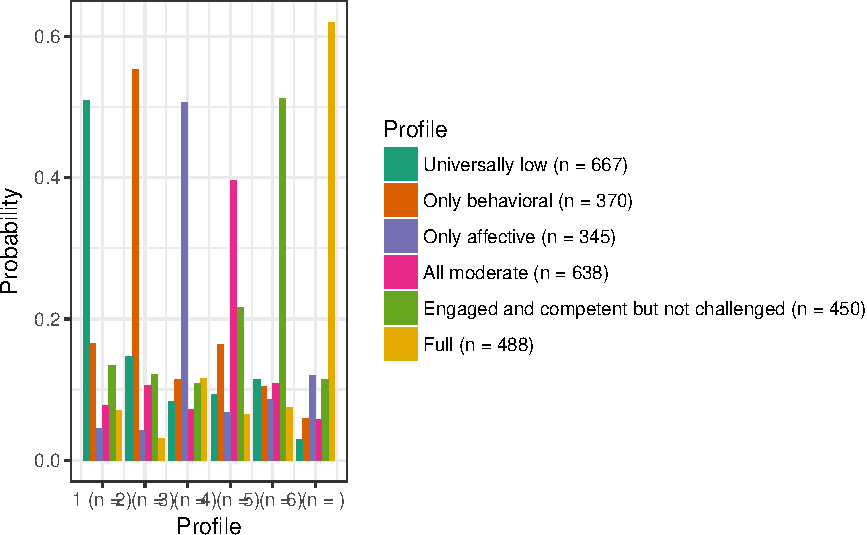
\includegraphics[width=1\linewidth]{rosenberg-dissertation_files/figure-latex/unnamed-chunk-12-1}

}

\caption{The six profiles of engagement (with variable values standardized)}\label{fig:unnamed-chunk-12}

{\centering 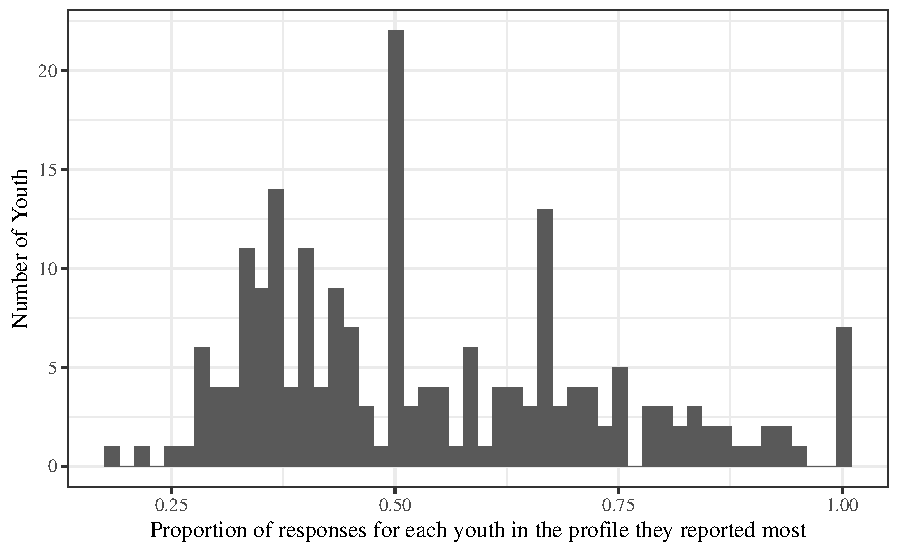
\includegraphics[width=1\linewidth]{rosenberg-dissertation_files/figure-latex/unnamed-chunk-13-1}

}

\caption{The six profiles of engagement (with raw variable values)}\label{fig:unnamed-chunk-13}
\end{figure}

The two plots are presented because they provide a different view into
the composition of the profiles: Those with the centered variables
highlights positive and negative departures from the mean value for each
variable, making differences between the profiles distinct. The plot
with the raw data instead highlights the reported values of the
variables, emphasizing the values of the variables in the profiles in
the same units that youth were asked to consider when they responded
(and potentially highlighting similarities that may seem very different
in the plot with the centered data).

The six profiles are characterized by both varying levels on both the
indicators of engagement (cognitive, behavioral, and affective) and
perceptions of challenge and competence. Also, the number of
observations across the profiles is relatively balanced (with no
profiles associated with a very large or small number of observations).
The universally low profile was associated with the most substantial
number of observations (\emph{n} = 667), followed by the all moderate
profile (\emph{n} = 638); each of the other four profiles was associated
with 300 to 400 observations. The results for research questions 3-5 use
this solution and the six profiles in subsequent analyses.

A MANOVA was carried out to determine whether the values of variables
differ across the profiles, with multiple ANOVAs used to determine which
variables (and for which profiles) there were differences. Note that for
the profiles (and their presentation in Figures 4.2 and 4.3 and Table
4.5), each response is associated with a probability of profile
membership at a particular moment. Because, across all responses, the
highest probability for each response was on average quite high (the
entropy statistic was .888), the highest probability was appropriate to
use to classify each response into one profile for the percentages and
results comparing the mean levels of each variable across profiles (with
a MANOVA). The MANOVA was statistically significant
(\emph{Pillai-Bartlett} = 0.633, \emph{p} \textless{} .001). The table
with the raw values, with subscripts indicating values \emph{the values
that were not statistically significantly different} is presented in
Table 4.5. Note that the \emph{F}-test associated each ANOVA was also
statistically significant. Descriptions of each the profiles taking
account of their size (in terms of the number of responses for which the
profile was most likely), their variable values, and what the profiles
suggest about youth engagement follow.

A \emph{universally low} profile consisted of a substantial proportion
of responses (22.55\%) was identified. This profile was characterized by
low levels of working hard, learning something new, and enjoying the
activity, and perceptions challenge and competence. For responses in
this profile, mean values were lower than their values in every other
profile for every variable except challenge, which was even lower in the
*engaged and competent but not challenged profile. Note that concerning
their raw values and not only their levels relative to the levels of the
variables for the other profiles, youth report very low levels (below
two on the one-four scale used) of all of the variables. In all, this
profile reflects very low levels of youth engagement during the specific
instructional episodes during which youth were signaled to respond.

An \emph{only behaviorally engaged} profile with a small proportion of
responses (12.51\%) was identified. This profile was characterized by
moderate levels of working hard, very low enjoyment of the activity, and
moderate levels of learning something new and challenge and competence.
The levels of reporting learning something new, challenge, and
competence were not distinguishable from those found in the responses
that make up the \emph{only affectively engaged} profiles. Levels of
working hard, an indicator for behavioral engagement, was higher than in
every profile except \emph{fully engaged} and \emph{engaged and
competent but not challenged}. These responses suggest that youth
perceive themselves to be working hard, but to not be enjoying what they
were doing and to not report learning something new, nor to be
particularly challenged or good at what they were doing when signaled.

An \emph{only affectively engaged} profile with a small proportion of
responses (11.66\%) was identified. This profile was characterized by
moderate levels of enjoyment, low levels of hard work, and moderate
levels of learning something new, challenge, and competence. Levels of
competence were the same as in the \emph{all moderate} profile. Youths'
reports of enjoying what they were doing at the time they were signaled,
an indicator of affective engagement, was higher than in every profile
except \emph{fully engaged} and \emph{engaged and competent but not
challenged}. When youth report this response, they enjoy what they were
doing, but were not working hard or learning something new, nor do youth
report being challenged by or good at the activity they were doing.

An \emph{all moderate} profile with a large proportion of responses
(21.57\%) was identified. This profile was characterized by moderate
levels of the three indicators of working hard, learning something new,
enjoying the activity, challenge, and competence. Levels of all of the
variables were, on average, lower for the responses that make up this
profile than among the responses associated with the \emph{engaged and
competent but not challenged} nor the \emph{full} engagement but were
still quite high on the one-four scale used. In sum, for youth reporting
\emph{all moderate} engagement were engaged, but may have the potential
to be more highly engaged (and challenged by and good at the activity).

An \emph{engaged and competent but not challenged} profile with a modest
proportion of responses was identified (15.21\%). This profile was
characterized by high levels of working hard, learning something new,
enjoying the activity, and competence, but low levels of challenge.
Levels of competence, enjoying, and working hard were identical between
the responses associated with this profile and the responses associated
with the \emph{fully engaged} profile, while levels of challenge were
very low: levels of challenge for these responses were lower than those
for every other profile. Levels of learning something new were slightly
lower than those in the responses that make up the \emph{fully engaged}
profile but were higher than their levels in the other four profiles.
This profile suggests youth can be highly engaged, while not being
challenged by the activity they were involved in at the time they were
signaled.

A \emph{full} profile with a modest proportion of responses (16.50\%)
was identified. This profile was characterized by high levels of working
hard, learning something new, enjoying the activity, challenge, and
competence. These responses reflect a very high level of engagement,
both relative to the other profiles and in absolute terms: All of the
mean levels were above 3.50, and, for working hard, youths' responses
averaged 3.96 on a one-four scale. Thus, when youth report engagement in
ways that were associated with this profile, the report being challenged
and good at what they were doing and, on the basis of these variables
and the indicators of engagement, were very highly engaged.

\begin{landscape}\begin{table}

\caption{\label{tab:unnamed-chunk-14}Raw variables values by profile}
\centering
\resizebox{\linewidth}{!}{
\begin{tabular}[t]{lrrrrr}
\toprule
Profile & Working Hard & Learning New & Enjoying & Challenge & Competence\\
\midrule
Universally low & 1.550$^1$ & 1.766 & 1.538 & 1.775 & 2.327\\
Only behavioral & 3.292 & 2.484 & 1.641 & 2.132 & 2.778\\
Only affective & 1.670 & 2.516 & 3.330 & 2.191 & 2.954\\
All moderate & 3.060 & 2.826 & 3.110 & 2.489 & 2.953\\
Eng. and comp. but not chall. & 3.909 & 3.487 & 3.822 & 1.276 & 3.604\\
Full & 3.959 & 3.801 & 3.881 & 3.742 & 3.631\\
\bottomrule
\end{tabular}}
\end{table}
\end{landscape}

\section{Results for Research Question \#3: What sources of variability
were there for the profiles of
engagement?}\label{results-for-research-question-3-what-sources-of-variability-were-there-for-the-profiles-of-engagement}

For all six profiles, the \emph{ICC}s (for the model with only the
youth, instructional episode, and program levels themselves, but not
variables at the levels) represent the systematic variability (the
proportion of variance explained) associated with each of the levels for
each profile. Thus, the different levels can have different proportions
of variance explained for different profiles, as presented in Table 4.6.
The systematic variability at the youth level, for example, could be .10
for the \emph{Full} profile and .025 for the \emph{Universally Low}
profile. At the program level, the \emph{ICC}s were found to be small,
with values ranging from 0.00 to 0.023, suggesting that little
variability can be explained by the program. For the instructional
episode level, the \emph{ICC}s were also small, ranging from 0.004 to
0.01. Finally, at the youth level, the \emph{ICC}s ranged from .093 to
.432.

\begin{table}

\caption{\label{tab:unnamed-chunk-15}Intra-class correlation (ICC) values for each of the three levels}
\centering
\begin{tabular}[t]{lrrr}
\toprule
Profile & Instructional Episode & Youth & Program\\
\midrule
Universally low (n = 667) & 0.006 & 0.267 & 0.023\\
Only behavioral (n = 370) & 0.006 & 0.093 & 0.009\\
Only affective (n = 345) & 0.004 & 0.262 & 0.003\\
All moderate (n = 638) & 0.015 & 0.310 & 0.000\\
Engaged and competent but not challenged (n = 450) & 0.009 & 0.100 & 0.000\\
Full (n = 488) & 0.031 & 0.432 & 0.019\\
\bottomrule
\end{tabular}
\end{table}

In terms of \emph{ICC}s at youth level across the six profiles, the
value for the youth-level ICC was highest for the \emph{Full} profile
(\emph{ICC} = .432), suggesting that some youth have a strong tendency
to be fully engaged (possibly due to their initial interest or other
individual characteristics and differences). The other profile
characterized by a consistent pattern across all of the variables--the
\emph{Universally low} profile--had a modest value for the ICC at the
youth level (\emph{ICC} = .267). Finally, a significant amount of
variability is associated with the residual (variance that was not
associated with the program, instructional episode, or youth levels).
This suggests that there is wide variation in youths' responses that may
not be readily explained or predicted by variables \emph{at one level
alone}. Remaining unexplained variability was captured by the residual
term. Some youth from particular programs may engage during some episode
instructional episodes in very high or low ways that were not captured
by modeling the variability at each of these levels alone.

The \emph{ICC}s lend insight into the sources of variability for a
specific profile; within-youth stability in terms of how frequently they
reported particular profiles could lend further insight by considering
variability across profiles. This analysis can be particularly useful
for understanding variability at the youth level, which the \emph{ICC}s
show to be associated with the most systematic variability. Each youth
has a most-frequently reported profile. Results show that for some
youth, the profile was very dominant, occurring in a substantial
proportion of youths' responses; for others, it occurs not that
frequently, meaning that youth report a variety of different profiles.

As presented in Figure 4.3, the mean proportion of responses for each
youth in the profile they reported most varied widely across youth.
Specifically, on average, youth reported their most-reported profile in
.540 (\emph{SD} = .194, \emph{min} = .182, \emph{max} = 1.00) of their
responses. There was a small number of youth who reported the same
profile in all of their responses, but for most youth, the profile they
reported most made up only a portion of all of their responses. For most
youth, the most common profile was observed just over 50\% of the time.
Note that any of the aspects of work with data versus none of the
aspects of work with data and the interactive effects of youth
characteristics were also examined. However, these were not found to be
statistically significant.

In sum, these findings show that there was substantial variability in
the profiles present at the youth level. Less variability was explained
by either the program youth were in or the nature of the particular
instructional episode present when youth were signaled. These results
set the stage for those for the next two research questions, on the
relations between the aspects of work with data (for research question
\#4) and the youth characteristics (for research question \#5) and the
profiles of engagement.

\begin{figure}

{\centering 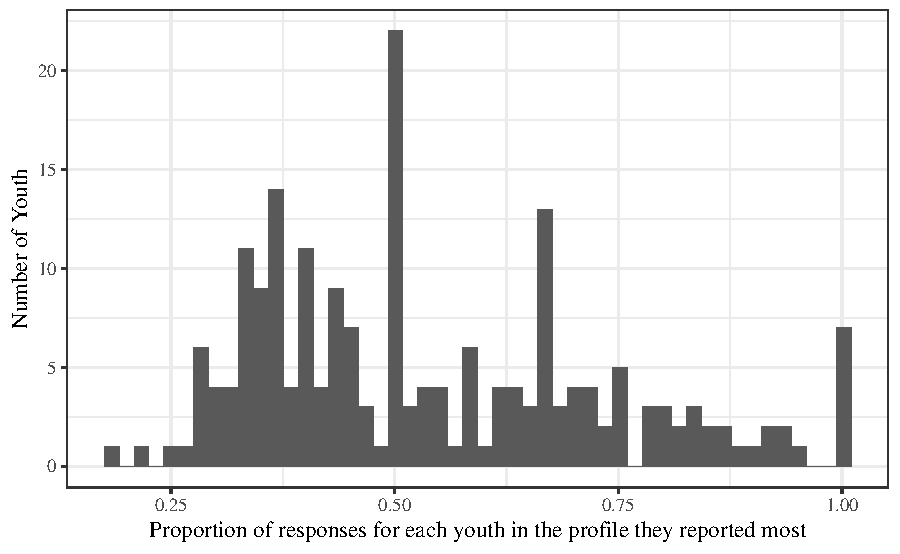
\includegraphics[width=0.8\linewidth]{rosenberg-dissertation_files/figure-latex/unnamed-chunk-16-1}

}

\caption{Histogram of the proportion of responses for each youth in the profile they reported most}\label{fig:unnamed-chunk-16}
\end{figure}

\section{Results for Research Question \#4: Aspects of work with data
and
engagement}\label{results-for-research-question-4-aspects-of-work-with-data-and-engagement}

To understand how aspects of work with data were related to engagement,
six analytic models were specified -- one for each engagement profile.
In each model, the dependent variable was the probability of a response
being classified in a particular profile (for example ``fully
engaged''), as determined by the Latent Profile Analysis. The five
aspects of work with data were the predictor (or independent) variables.
Varrious aspects of work with data tended to co-occur and so
simultaneously entering indicators for all five aspects served to
isolate the association for any single aspect, while controlling on the
presence of the others. All models also include some youth
characteristics which will be used to answer research question five
below.

Associations between the five aspects of work with data and the six
engagement profiles are presented in the bottom half of Table 4.7. In
this table, each column represents the output from one of the six
different models. As an example, the first column reports the
coefficients for the associations between the predictor variables and
the \emph{Only behavioral} profile. Because the outcome was in the form
of a probability (ranging from 0.00 to 1.00), it can be interpreted as
the change in the probability of a response being associated with each
profile. Note that the \emph{p}-values were calculated using the most
conservative and recommended by recent research Kenward-Rogers
approximation (Halekoh \& Hojsgaard, 2014).

The only engagement profile that was significantly associated with any
aspects of work with data was the Full profile (see the column with the
column name Full for these results). When program activities involved
modeling data, youth were around 3\% more likely to be fully engaged
(\(\beta\) = 0.034 (0.017), \emph{p} = .020; partial \(R^2\) = .002). In
other words, when program activities included modeling data, youth were
more likely to report working harder, learning more, enjoying themselves
more, and feeling more competent and challenged.

Youth were also more likely to be in the Full engagement profile when
program activities included generating data (\(\beta\) = 0.027 (0.015),
\emph{p} = .033; partial \(R^2\) = .002). These particular program
activities increased the probability of full engagement by around 3\%.
To sum up these two findings, modeling data and generating data were
associated with a (very) positive form of engagement, that exhibited by
the Full profile. However, the effect sizes indicate quite small effects
in substantive terms. Note that the interactions between the individual
aspects of work with data and youth characteristics were interacted.
However, none of these relations were found to be statistically
significant.

Sensitivity analysis was carried out for the statistically significant
two effects was carried out to determine just how robust they were. This
follow-up analysis revealed that the effect of modeling data on
\emph{Full} engagement much more robust than that for generating data:
9.835\% of this effect (of data modeling) would have to be due to bias
to invalidate the inference about its effect. For generating data, only
1.884\% of the effect of generating data would need to be due to bias to
invalidate the inference about its effect. These values were not
minuscule but were also not very large (Frank, 2003). So, while
statistically significant, the effect of data modeling seems to be a
more robust effect than the effect of generating data, which does not
seem to be a very robust (and should, therefore, be interpreted with
some caution).

\begin{landscape}\begin{table}

\caption{\label{tab:unnamed-chunk-17}Results of mixed effects models with the interactions between interest and other characactistics and the composite for work with data}
\centering
\resizebox{\linewidth}{!}{
\begin{tabular}[t]{lllllll}
\toprule
Profile & Universally low $\beta(\textit SE)$ & Only behavioral $\beta(\textit SE)$ & Only affective $\beta(\textit SE)$ & Eng. and comp., not chall. $\beta(\textit SE)$ & All moderate $\beta(\textit SE)$ & Full $\beta(\textit SE)$\\
\addlinespace[0.3em]
\multicolumn{7}{l}{\textbf{Youth characteristics}}\\
\hspace{1em}Pre-interest & -0.047 (0.022) & -0.013 (0.012) & -0.012 (0.019) & 0.039 (0.016)* & 0.007 (0.01) & 0.018 (0.021)\\
\hspace{1em}Gender-Female & 0.06 (0.037)+ & 0.019 (0.019) & -0.038 (0.033) & 0.025 (0.028) & -0.02 (0.018) & -0.035 (0.037)\\
\hspace{1em}URM status & -0.01 (0.052) & 0.031 (0.026) & -0.076 (0.046) & -0.012 (0.04) & 0.018 (0.025) & 0.043 (0.053)\\
\addlinespace[0.3em]
\multicolumn{7}{l}{\textbf{Aspects of Work With Data}}\\
\hspace{1em}Asking & -0.015 (0.018) & 0.015 (0.015) & 0.023 (0.017)+ & -0.011 (0.015) & 0.004 (0.014) & -0.019 (0.016)\\
\hspace{1em}Observing & 0.003 (0.018) & 0.013 (0.015) & 0.007 (0.017) & 0.009 (0.015) & -0.017 (0.014) & -0.025 (0.016)\\
\hspace{1em}Generating & -0.014 (0.017) & 0.014 (0.014) & 0.012 (0.016) & -0.014 (0.014) & -0.02 (0.013) & 0.027 (0.015)*\\
\hspace{1em}Modeling & 0.004 (0.019) & -0.023 (0.016) & -0.004 (0.018) & 0 (0.015) & -0.012 (0.015) & 0.034 (0.017)*\\
\hspace{1em}Communicating & 0.002 (0.018) & 0.018 (0.015) & -0.011 (0.017) & 0.004 (0.015) & 0.016 (0.014) & -0.027 (0.016)\\
\bottomrule
\end{tabular}}
\end{table}
\begin{flushleft}\emph{Note}. *: \emph{p} \textless{}.05; +: p \textless{} .10\end{flushleft}
\end{landscape}

\section{Results for Research Question \#5: Youth characteristics and
engagement}\label{results-for-research-question-5-youth-characteristics-and-engagement}

Associations between youth characteristics and the six profiles are
reported in the top half of Table 4.7. Youth who enter the program with
higher levels of interest (in STEM) were more likely to report being in
the engaged and competent but not challenged profile (\(\beta\) = 0.039,
\emph{p} = .009; partial \(R^2\) = .001). In other words, youth who were
more interested at the outset of the program report working harder,
learning more, enjoying themselves more, and feeling more competent when
they were involved in program activities, though they also report lower
levels of challenge. For this effect, 17.879\% would be needed to
invalidate the inference, suggesting a moderately robust effect.

In terms of youths' pre-program interest, these analyses show that youth
who enter the program with higher levels of interest (in STEM) were more
likely to report being in the \emph{Engaged and competent but not
challenged} profile (\(\beta\) = 0.039, \emph{p} = .009; \emph{partial
\(R^2\)} = .001). For each one-unit increase in pre-program interest in
STEM, youth were around 4\% more likely to report this profile. In other
words, youth who were more interested at the outset of the program
report working harder, learning more, enjoying themselves more, and
feeling more competent when they were involved in a program's
activities, though they also report lower levels of challenge. For this
effect, 17.879\% would be needed to invalidate the inference, a slightly
larger value for the follow-up sensitivity analysis than those found for
the (statistically significant) relations involving the aspects of work
with data, suggesting a moderately robust effect.

There were not any statistically significant effects of youths' URM
status. This lack of relations between URM status and youth engagement
may be a function of the large proportion of youth from
under-represented (in STEM) racial and ethnic groups. Hispanic (48\%),
African American or Black (36\%), and youth who identify as being from
multiple racial and ethnic groups (3\%) made up 87\% of the youth in the
programs, so there were not many youth \emph{not} from under-represented
groups in the sample, suggesting that the absence of findings may be due
to this small sample (and low statistical power). Nevertheless, no
relations between URM status and youths' engagement were found,
indicating that there is at least no evidence that youth from such
backgrounds do engage in different ways.

These (somewhat minimal) findings for the youth characteristics were
more surprising than those observed for the aspects of work with data.
The results of research question \#3, on the sources of variability for
the profiles of engagement, suggested that there was much systematic
variability at the level of the youth (there were large \emph{ICC}s at
the youth level, with smaller \emph{ICC}s at the instructional episode
level). Because pre-interest, gender, and URM status were variables at
this level, it could be expected that they would have meaningful
relations with the profiles of engagement. However, it appears that the
particular youth characteristics considered were not useful at
explaining much of this variability; possible reasons why are discussed
further in the next section.

\chapter{Discussion}\label{discussion}

Each of the disciplines that contribute to STEM learning - science,
technology and computer science, engineering, and mathematics - involve
work with data. In this study, engagement was used as a lens to
understand the experience of youth working with data during summer STEM
programs. In particular, five aspects of work with data, a) asking
questions, b) observing phenomena, c) constructing measures and
generating data, d) data modeling, and e) interpreting and communicating
findings, were occurred regularly in the programs. There were some
examples of ambitious activities centered on working with real-world
data as well as some that highlight substantial heterogeneity in how
work with data was enacted.

I identified six profiles of engagement using LPA. These profiles
represented different configurations of how youth were working hard,
learning, enjoying themselves, and feeling challenged and competent at
the time they were signaled as part of the ESM approach. Relations of
the five aspects of work with data and youth characteristics
(pre-program interest in STEM and youths' gender and status in terms of
being a member of under-represented groups in STEM) were, overall, not
strongly related with the profiles of engagement, though some key
findings were identified. Generating and modeling data were both related
to the most potentially beneficial profile (full engagement), one
characterized by high levels of all five of the engagement variables.

This study suggests that work with data and contemporary engagement
theory as interpreted in this study can serve as a frame to understand
what youth do in summer STEM programs. These findings also show the
value of an innovative method, ESM, and an analytic approach designed to
identify engagement holistically, LPA, that together to provide some
access to youths' experience in-the-moment of the activities they were
involved in during the program. Data, and how youth and students in K-12
settings can themselves work with data, is an important, yet perhaps
under-emphasized part of STEM learning. In the remainder of this
section, I discuss key findings with respect to a) work with data, b)
youths' engagement, and c) what relates to youths' engagement. Also,
some limitations and recommendations for future research as well as
implications for practice are identified and described.

\section{Key findings related to work with data in summer STEM
programs}\label{key-findings-related-to-work-with-data-in-summer-stem-programs}

Results showed that work with data was common in the summer STEM
programs. There was variability in \emph{which} aspects of work with
data was present: Making observations, in some form, occurred during
24\% of the program's time, for example, while generating data and
communicating findings both occurred more frequently, during 43\% of the
instructional episodes. These findings, broadly, suggest that work with
data occurred enough that we might expect to see differences in youths'
engagement. They align with what may be expected given past research:
Such programs are designed to engage youth in the practices, including
and as I argued earlier \emph{especially} those relating to work with
data, of STEM domains (Dabney et al., 2012; Elam et al., 2012). Even
still, these are the first results of this kind (in terms of the
proportion of the time spent in the programs). Using video-recording
data and a sampling strategy that can provide insight into the amount of
overall time spent was an important component of achieving these
findings. While there are no other results of this particular kind, a
related, an area of related work concerns other studies that have used
the PQA measure. Some research reports call for greater use of measures
(such as the PQA) in the study (and evaluation) of summer and
outside-of-school STEM programs (e.g., Yohalem et al., 2005). As one
example of such a study that used the PQA (but one that is not focused
on STEM), Smith et al. (2012) reported findings from a continuous
improvement intervention, finding that the intervention positively
impacted the quality of instruction in the programs.

In addition to work with data being common, I found it was highly varied
in how it was enacted. In the course of the four-week summer STEM
programs, youth engaged in what can be described as ambitious, specific,
and potentially highly engaging ways of being involved in work with
data. For example, when generating data, many times (in 47\% of the
episodes that involved this aspect) youth recorded their observations;
when modeling data, youth were involved (in 72\% of the episodes) in the
use of statistical and mathematical models of real-world phenomena. When
interpreting and communicating findings, youth regularly (during 48\% of
episodes) had opportunities to share (with other youth in the program)
what they found or created as a result of their earlier investigations
or work.

What occurred during the \emph{rest of the program's} time was also
notable. When youths' questions, for example, were not focused on
predicting or hypothesizing about what they were exploring, the type of
question was more general, or was instructor-led, rather than driven by
youth. These instructor-driven forms of work with data were not aligned
with recent reform efforts (i.e., National Research Council, 2012; NGSS
Lead States, 2013; National Governors Association Center for Best
Practices, Council of Chief State School Officers, 2010), but could be
expected given past research pointing out variability in what evidence
and data mean, especially in science education settings (McNeill and
Berland, 2017; Lehrer \& Schauble, 2015). Also of note was the frequency
of these three aspects of work with data overall: They occurred much
more frequently than the two (making observations and data modeling) for
which a larger proportion of their enactment was more in-line with
policy and curricular standards. The type of activities that may be the
most demanding for youth was still common (and may spark youths'
engagement) but was not quite as common as the overall frequencies
presented for the quantitative would suggest.

Past research does point out a heterogeneity in how work with data was
enacted in education similar to that found in this study. For example,
Hancock et al. highlight the use of ``data to solve real problems and to
ask authentic questions'' ( p.~337). Research on generating data
emphasized an aspect not very much the focus of the present research,
namely, structuring data into spreadsheets (Konold, Finzer, \& Kreetong,
2017; Lehrer \& Kim, 2009). This suggests a reason why youth were able
to ask questions and ideas for how they might do so more: Make
activities in summer STEM program youth-centered, rather than
instructor-centered. Research on the data modeling aspect of work with
data highlights the use of statistical models much more than the
physical models which were sometimes found to be a way in which youth
engaged in data modeling (Petrosino, Lehrer, \& Schauble, 2003; Lesh,
Middleton, Caylor, \& Gupta, 2008; Lee, Angotti, \& Tarr, 2010).
Nevertheless, many of the ways youth engaged in data modeling aligned
with this past research, particularly when the goal of the activity was
to model variability. This past research that encouraging youth to
consider summaries of data, such as the mean and standard deviation, may
be a promising way for them to engage more deeply in data modeling
(Lehrer, Kim, \& Schauble, 2007; Lehrer \& Schauble, 2004). In this way,
some (but not all) of the aspects work with data aligned with past
research; when they align, they are encouraging, and when they do not, I
present some ideas for how to involve youth in more engaging aspects of
work with data.

\section{Key findings related to
engagement}\label{key-findings-related-to-engagement}

Six profiles of engagement were found using a rigorous model selection
approach. It is important to note that LPA is an exploratory approach:
The number and nature of the profiles identified were found through a
rigorous and systematic approach, but this is not a guarantee that the
same number and make-up of profiles would emerge in other samples and
other contexts: These profiles should be considered as initial evidence,
and not as proof that these are \emph{the} six profiles of engagement
that will exist in all settings. The number of profiles found is broadly
similar to that found in past research. Six is the same number of
profiles of engagement identified in recent, past research and the
similar number provides further information about the nature of
engagement in educational contexts: Schmidt et al. (2018) found six
profiles of engagement. Their profiles were constructed on the basis of
the indicators (cognitive, behavioral, and affective) of engagement, and
not perceptions of challenge and competence.

As Schmidt et al.`s study is the only other to examine engagement
profiles, another point of comparison is other outcomes that are
different from but related to engagement, such as youths' (and
students') achievement goals (see Wormington and Linnenbrink-Garcia,
2017, for a review in educational settings). Wormington and
Linnenbrink-Garcia (2017) report that, usually, a smaller number, with
only two of the 22 studies reviewed finding six profiles of goals. This
suggests, on the basis of this study and Schmidt et al.'s (2018) study,
that there may be a greater variety of types of engagement exhibited
than, for example, types of achievement goals. However, in addition to
the different construct, the engagement profiles were constructed on the
basis of data collected via ESM, while the achievement goal profiles
were constructed on the basis of self-report surveys and not via ESM.
Knowing the number of profiles found when profiles are used to explore
various constructs is potentially helpful, additional information about
how engagement was experienced by youth. In addition, the greater number
of groups may suggest that engagement, explored through ESM, may
demonstrate more variability in terms of how its constituent parts are
experienced together and at once. Exploring whether this greater
variability was due to the method of data collection (ESM or
self-report), the construct (engagement or achievement goals), or some
other reason.

In terms of comparing the make-up of the specific profiles to other,
past research, little work has examined profiles of engagement. Schmidt
et al. (2018) did examine profiles of engagement, which were constructed
from indicators cognitive, behavioral, and affective engagement (but not
perceptions of challenge and competence, as in this study). Schmidt et
al. (2018) found six profiles, some of which partially overlap with
those found in the present study. In particular, on the basis of the
items shared between the studies, a \emph{Universally low}, \emph{All
moderate}, and \emph{Full} profile were found in both studies. However,
as these profiles are characterized by the (uniform) level across all of
the variables, this is only limited evidence for the presence of these
profiles in the larger population of youth engaged in science and
STEM-related learning activities.

The six profiles lend insight into how youth engage during summer STEM
programs. In particular, the \emph{Only behavioral}, \emph{Only
affective}, and \emph{Engaged and competent but not challenged} profiles
were found in the present study, but not in Schmidt et al.'s (2018)
study. Youth were highly engaged (as may be anticipated given the goals
and design of such programs), but perceive a misalignment between their
(high) competence and how (not very) challenged they were. According to
past theory (e.g., Csikszentmihalyi, 1997) and some research (e.g.,
Shernoff et al., 2016), such a profile would be unexpected, as high
levels of engagement are expected to be associated with high levels of
\emph{both} challenge and competence. In this study, a profile
characterized by high competence but (very) low challenge was associated
with very high engagement. This profile, \emph{Engaged and competent but
not challenged}, then, seems to suggest a type of engagement that may be
unique and common to summer STEM programs. Perhaps such a profile may be
expected given the lower stakes (compared to formal educational
settings) of summer STEM programs (and other informal learning
environments) and the degree of competence that youth--many of whom have
chosen to attend the particular program (Beymer et al., 2018)--perceive
during them.

In addition to suggesting a profile of engagement that is distinct to
summer STEM program, this profile and the other two not found in past
research have some implications for youth activity leaders. In
particular, they suggest that lower challenge may \emph{not}, as would
be anticipated given theory and past research, be associated with lower
engagement. Because of this, it may be recommended that activities that
are not challenging but have other possible benefits to youth (i.e.,
benefits from activities designed to support youths' social skills), can
be integrated into programs, along with other, more challenging
activities that are also highly engaging to youth.

These profiles have some implications for the study of engagement. They
also have some implications for the analysis of multidimensional data on
engagement. First, they suggest that perceptions of challenge and
competence be considered in future research. This is because some of the
profiles were distinguished on their basis. This approach also may be
more parsimonious than including perceptions of challenge and competence
as separate predictors (i.e., Shernoff et al., 2003). In addition to
these empirical reasons, past research on engagement (i.e.,
Csikszentmihalyi, 1990) and on the profile approach (Bergman \&
Magnusson, 1997) suggest that they are theoretically inseparable from
engagement, another reason for modeling them as they were modeled in the
present study. These implications, then, are specific to the study of
engagement but also highlight some of the potential of the profile
approach, as well.

\section{Key findings related to work with data and youth
characteristics and their relations to
engagement}\label{key-findings-related-to-work-with-data-and-youth-characteristics-and-their-relations-to-engagement}

In line with what the sources of variability would suggest, relations
between work with data were minimal, though some small, statistically
significant relations were identified. The question of whether and how
work with data relates to engagement has not been the focus of past
research on work with data. This past research has focused more on very
specific cognitive outcomes, designs (often from design-based research)
for work with data, and the challenges teachers and learners may
anticipate when they are involved with particular aspects of work with
data, particularly data modeling (and accounting for variability in
data). Given the absence of research from an engagement perspective,
these are new findings that suggest, in this context, that work with
data may not be strongly related to engagement in educational contexts.

Why might these relations be so minimal? First, and foremost, the small
amount of variability at the instructional episode level (see the
\emph{ICC}s for this level reported for in the results for research
question \#3) was critical because it means that few relations between
variables at the instructional episode level were anticipated (on this
basis). In particular, very small amounts of variability at the
instructional episode level was found for all six profiles of
engagement, and these values were smaller than those found in the one
other past study that employed the same analytic approach (Strati et
al., 2017). This is an important consideration in terms of the null
findings because it suggests that there was very little systematic
variability \emph{at the level that work with data was at, the
instructional episode} to be explained. This may be due to the summer
stem setting. Perhaps youth were less likely to engage differently from
instructional episode to instructional episode (compared to in K-12
educational settings) because there was less variability in what took
place across the episodes. Youths' tendency to not engage different from
instructional episode to instructional episode (in systematic ways) may
also be because youth perceive there to be lower stakes for the
programs' activities and therefore do not perceive the changes in the
instructional episode as a factor that impacts their engagement. This
consideration is described in greater detail in the limitations section.
There are other possible reasons, though, too, for the minimal
relations. One may be that work with data was \emph{not}, as carried out
in these summer STEM programs, very engaging, even accounting for the
small amount of variability at the instructional episode level. Another
possibility is that the novel analytic approach or the measures used
also had impacts. But, again, the small variability at the instructional
episode level was likely a greater factor than these, and a review of
the correlations between the aspects of work with data and the variables
used to create the profiles showed minimal relations. These two
potential explanations are explored further in the next section, on
limitations to the present study and recommendations for future
research. Taken together, it seems that the major reason for limited
relations between work with data and youth engagement was that youth did
not engage very differently (in systematic ways) from instructional
episode to instructional episode.

Even so, there were \emph{some} noteworthy findings that could be
anticipated on the basis of the importance of the two aspects of work
with data that were found to relate positively to youths' engagement. In
particular, both generating and modeling data were found to be
positively (and statistically significantly) related to the \emph{Full}
profile, suggesting that when youth were involved in these practices,
then they were more likely to be highly engaged. In particular, given
the makeup of this profile, this suggests that when youth were involved
in these aspects of work with data, they were more likely to report high
levels of cognitive, behavioral, and affective engagement, and high
perceptions of competence and challenge. Generating and modeling data
may have such relations because they were particularly important aspects
of work with data. As Lehrer and Schauble (2006) explain,
\emph{inscriptions serve commitments}: Choosing to record an observation
or an idea as data involves the process of identifying something that is
worth recording and then recording the parts that are of interest. Thus,
generating data may be fully engaging to youth because it is, generally,
demanding and important with respect to work with data. Modeling, too,
is an important practice. It has been described as \emph{the} central
scientific and engineering practice (Lehrer \& Schauble, 2015; Weisberg,
2012), and its relations with full engagement provides some actionable
evidence for its importance in the context of summer STEM programs.
Modeling may be especially engaging to youth because such work positions
learners as the creators of new information, in addition to using models
created by others to learn about authoritative sources of information.
This is one of the key affordances of modeling in teaching and learning
contexts (Berland et al., 2016; Schwarz et al., 2009). Moreover, when
learners create new knowledge (including doing so through the use of
data modeling), they can begin to shape not only what knowledge learners
construct, but also how they construct it, a challenge in science
education contexts (Miller et al., 2016) and likely in other STEM
content areas, we well.

The null findings for the relations of asking questions, making
observations, and interpreting and communicating findings were
noteworthy, too. They suggest that, if these aspects of work with data
were (positively or negatively) related to youths' engagement, then
their effects were not large enough to be detected. They may not be able
to be detected for a number of reasons: simply because they were very
small given all of the other factors that impact youths' engagement,
because the aspects of work with data were enacted in a myriad of ways
which may be more or less engaging, and because they simply were not as
engaging. Nevertheless, future research may seek to understand why these
aspects did not relate to engagement.

As there is no research on how work with data relates to youths'
engagement, the findings associated with this research question provide
some initial evidence for how some aspects of work with data relate to
youths' engagement. These findings suggest that these activities may not
be more engaging \emph{per se}. Instead, it may be the way that youth
engage in them that matters, in alignment with past research (Berland et
al., 2017). While the findings for this question were somewhat minimal,
there are key findings from both the important relationships that were
found to be statistically significant (between generating data and data
modeling and \emph{Full} engagement) and from those that were not. Other
samples, other enactments of work with data, and, possibly, other
analytic approaches can build on this work to further substantiate what
is known about how work with data engages youth and other learners.

Why were there such limited findings in terms of relations between
youths' characteristics and youths' engagement? There was a lot of
variability in the profiles of engagement at the youth level, but there
were not many relations in terms of youths' gender, URM status, or
pre-program interest. Given past theory and research have suggested that
learners' gender, URM status, and individual or pre-program interest can
predict engagement (Bystydzienski, Eisenhart, \& Bruning, 2015; Hidi \&
Renninger, 2006; Shernoff \& Schmidt, 2008). Despite these surprising
findings, youth with higher pre-program interest were found to be more
likely to be \emph{Engaged and competent but not challenged}. This
suggests that youth with a higher interest in STEM were inclined to be
highly engaged and good at what they were doing, but were not challenged
by the activities they experience. This finding is in line with past
research suggesting a relationship (direct or as a moderator) between
youth characteristics (including interest) and their engagement
(Shernoff et al., 2003; Shernoff et al., 2016; Strati et al., 2017).
More specifically, this finding suggests that for youth who were
particularly interested (and those who choose to attend) summer STEM
programs, what they were involved in may not challenge them very highly.
This finding has implications for past research that shows youth who
choose to attend summer STEM programs were more engaged (but that does
not speak to their degree of challenge; Beymer, Rosenberg, Schmidt, \&
Naftzger, 2018).

While the findings for this research question, like those for the
relations between the aspects of work with data and youths' engagement,
they provide some information about how these characteristics relate to
youths' engagement. Knowing that youth who were more interested before
the beginning of the summer STEM programs were more likely to be working
hard, learning something new, and enjoying what they were learning, and
perceive themselves to be good at what they were doing but not
challenged, is novel. Moreover, the null findings suggest that other
characteristics, including those measured but not included for this
analysis (such as youths' pre-program perceptions of their competence)
as well as those not measured at all, may be considered in follow-up
studies and future research. While the programs that were involved in
the study have many affordances for work with data and for being highly
engaging for youth, they have some limitations, too, particularly with
respect to support work with data. Importantly, these were not programs
explicitly designed to support work with data; while such contexts are
being developed, they are not yet widespread. Moreover, youth may
perceive the programs to have lower stakes in terms of their future.
This may mean that the individual activities that youth engage in were
less connected to their engagement: Youth instead engage in typical (to
each youth) ways, rather than in ways that were much more sensitive to
changes in their context. Another possible explanation for these limited
findings may be that youth were not very challenged or were not very
supported. A profile with low challenge but high competence and
cognitive, behavioral, and affective engagement was found, suggesting
that youth may be engaged and good at what they were doing, but were not
challenged: Greater challenge may be found to be associated with more
\emph{full} engagement, for example.

\section{Limitations to the present study and recommendations for
research}\label{limitations-to-the-present-study-and-recommendations-for-research}

To sum up the previous sections, work with data was frequent but varied
in how it was enacted and profiles of engagement representing different
and interpretable configurations of five engagement-related variables
were found, but work with data and youths' characteristics were not
found to be very strongly related to any of the profiles. Some
limitations to the study that may provide insight into why such minimal
relations to the profiles were found and into other findings are
detailed in this section.

First, the programs participating in this study were not designed
especially to support youth in work with data. Instead, the programs
were designed around best practices for summer STEM programs to support
youth to engage in a wide variety of STEM-related practices--and in
other activities, such as those intended to build a sense of camaraderie
among the youth in the programs. In this study, aspects of work with
data were identified and were found to be common, but some of the
heterogeneity in the nature of working with data may be due to this
reason: Planning and instruction for the programs did not aim to foster
rich work with data any more than the other activities (STEM and
otherwise) that made up their programming. In addition to the varied
ways in which youth worked with data, some of the relations of the
variables for the five aspects of work with data to youths' engagement
may be due to the ways that the variables for work with data indicated,
in fact, many different ways of working with data. Some of these aspects
of working with data, particularly those that were highly-specific with
respect to how the data was involved and to how focused and sustained
the work with data-related activity was, may be more engaging to youth
than the others, such as those that were more general,
instructor-focused, or brief. These two types of working with data were
considered the same in the variables used to predict youths' engagement.
Future research can aim to understand youths' engagement in
outside-of-school data science programs and K-12 units, for example,
that are focused more on work with data to understand better how work
with data engages youth. Nevertheless, this study does provide insight
into how work with data took place during \emph{model} (i.e., designed
around best practices for such programs) summer STEM programs and how
such work relates to youths' engagement.

In a related point, it is important to point out that while
outside-of-school STEM programs have affordances, they also have some
distinct features as well as some limitations. One of their key features
is their duration: As in this study, youth were involved over a
substantial, but still limited period of time (around four weeks).
Another feature concerns the nature and quality of the teaching (and
learning) that take place during them. The contexts (including in the
field) in which youth were engaged good spark their engagement and could
support work with data better than some K-12 learning environments. They
also have some key limitations, including the possibility that youth
considered their time in them to be enjoyed and to be social, meaning
that the way they engaged in the programs as documented in this study
could be unique to outside-of-school STEM programs like those in this
study. In particular, the \emph{engaged and competent but not
challenged} profile may be unique to learners in summer STEM programs.
This is a limitation in addition to those documented earlier, namely,
that the limited variability at the instructional episode level may also
be due to the lower stakes that learners in these contexts may perceive.

Learning environments that deliberately support work with data over an
extended period may demonstrate different patterns of engagement. One
key reason why this may be is the importance of work with data being
part of a cycle (and how this cycle often did not take place in these
outside-of-school STEM programs). Nevertheless, in addition to
illustrating the nature and frequency of work with data, the open-ended,
qualitative coding carried out for research question \#1 also provided a
lens into how work with data was (or was not) sequenced. There were
instances of youth activity leaders linking earlier to later activities.
For instance, the mathematics-focused programs, such as the
\emph{Adventures in Mathematics} program, the youth activity leaders,
recognizing that youth had difficulty solving equations, used duct
tape--and building on an earlier activity in which youth considered what
constituted a rate--asked youth to count how many ``hops'' it would take
someone to move from one end of a line of duct tape to the other. The
youth activity leader than asked youth to consider how far they could
move in one hop and to consider how they could find out many hops it
would take, using a mathematical equation. In this activity, youth were
supported in their attempts to approach mathematics problem-solving by
linking data modeling to an earlier activity that involved generating
data about the number of hops.

Other instructional episodes evidenced fewer connections between earlier
and later activities and also the opportunity for more sustained
involvement in work with data. For example, during some instructional
episodes, youth-generated data, but they did not use the data they
generated in subsequent activities. In the engineering-focused programs
(\emph{Uptown Architecture}, \emph{Crazy Machines}, and \emph{Dorchester
House} particularly, youth often generated data that resulted from their
engineering designs (and communicated and interpreted their findings,)
but did not model this data as a regular part of their activities. In
one particular example, in the \emph{Ecosphere} program, youth collected
water samples in the field. They then brought these samples to the
classroom and tested the water, involving youth in both collecting and,
to a degree, generating data (by noting the pH levels of the water).
However, later in the day, youth created a small-scale model (with
inclined trays of dirt, rocks, and plants) of an ecosystem, in which
they added food coloring to determine the impacts of chemicals and acid
rain. Youth then interpreted and discussed these findings, but did not
connect the discussion to the water samples youth collected and tested
earlier. While these specimens were collected to serve as data for
future activity, there was no generating data observed during the
episode. In other instances, youth were involved in observing phenomena
but were not ever asked to use those data in subsequent activities. How
this sequencing of work with data may impact youths' engagement was not
considered in this study, though past research suggests that this factor
may make work with data more (or less) engaging and impactful to
learners. As McNeill and Berland (2017) argue, it is not just engaging
in these practices by rote, but about integrating them, as they overlap
and interconnect. They argue that a view of work with data focused on
``making sense of'' data generated from real-world phenomena, as well as
sustained engagement in work with data involving the revision of
earlier, intermediate ideas, are important considerations regarding the
enactment of work with data.

In addition to limitations related to the focus of the programs and how
work with data was enacted as part of a cycle, there were also some
general measurement-related limitations. Work with data can be difficult
to measure because, as the qualitative analysis revealed, there were a
variety of ways in which youth can be involved in work with data.
McNeill and Berland (2017) describe a similar type of disagreement
across science education settings: While a limitation, the coding frame
did represent agreement across a range of studies across STEM contexts
for the aspects of work with data. In terms of the alignment of the
measure with the conceptual framework for work with data, the dimensions
of the STEM-PQA measure aligned closely with the aspects of work with
data. However, there were some divergences that may have had an impact
upon some of the findings. For example, for the interpreting and
communicating findings code, the STEM-PQA codes for \emph{Analyze}
(``Staff support youth in analyzing data to draw conclusions'') and
\emph{Use symbols or models} (``Staff support youth in conveying STEM
concepts through symbols, models, or other nonverbal language'') were
used. In the case of the latter STEM-PQA code, conveying STEM concepts
through symbols, models, or other nonverbal language could have
reflected instructional episodes in which youth used, for example,
mathematical equations or formulas, but did not do so as part of
modeling data of a phenomena in the world: They could have simply been
using an equation outside of the context of any particular phenomena.
Future research may consider the usefulness of coding for this aspect of
work with data (and this aspect of science curricular standards in
particular; see NGSS Lead States, 2013).

As another example of this limitation related to how work with data was
measured, generating data was an aspect of work with data that the
open-ended qualitative analysis revealed to be less associated with less
systematic groups of practices, or themes, than the other aspects. The
STEM-PQA codes corresponding to this aspect of work with data were
\emph{Collect data or measure} (``Staff support youth in collecting data
or measuring'') and \emph{Highlight precision and accuracy} (``Staff
highlight value of precision and accuracy in measuring, observing,
recording, or calculating''). Particularly in the case of the latter
code, the emphasis on precision and accuracy may have been outside of
activities focused on recording data or creating coding frames. Future
research may consider a coding frame that is (more) focused on
generating data, though considerations of precision and accuracy are key
aspects of doing so, and so perhaps separating the act of generating
data from considerations that are important to keep in mind while doing
it may be a promising direction for future research. While these
divergences in measures were not large, they suggest that the coding
frame for work with data is a limitation of the present study.

It is possible that the somewhat minimal findings are, in part, a result
of the analytic approach. A similar mixed effects modeling approach has
only been used in one other study (Strati et al., 2017), and that
approach did not use profiles (as in this study) as the outcome. In this
study, little variability at the instructional episode level was found,
and so minimal relations between factors at this (instructional episode)
level and the profiles of engagement was expected. Might profiles, but
not the variables used to create them, be less variable at the
instructional episode level? One way to consider such an alternate
explanation is to use the data used in this study as part of
correlational analyses, or another analysis that uses that variables
used to create profiles of engagement but does not use the profiles
themselves. By removing some of the complexity of both the sample
(accounted through the youth, the instructional episode, and the program
groups, which were modeled as random effects) and the profile approach,
may present a clearer set of relations between work with data and youth
characteristics and the five variables for engagement: Examining them,
in Table 4.2, suggests that the analytic approach was not the primary
factor in terms of explaining the minimal relations, as none of the
correlations between the variables used to create the profiles and the
aspects of work with data was greater than \emph{r} = .05 (in absolute
values). Nevertheless, such an approach is less conservative than the
modeling approach because the groups in the data would not be accounted
for in ways that are recommended (Gelman \& Hill, 2007). Related to
pursuing a different approach to the data analysis, other outcomes from
working with data may also show different (and more strongly positive or
negative) relations. Such outcomes may be at the instructional episode
level, like engagement, or may be longer-term, like youths' future goals
and plans after the conclusion of programs.

\section{Implications for Practice}\label{implications-for-practice}

A few implications for practice can be drawn from this study, though
these are somewhat restricted given the minimal findings. First,
\emph{generating data} and \emph{modeling data} in particular may be
beneficial in terms of engaging youth. Youth activity leaders (in summer
STEM and other STEM enrichment contexts) and teachers (in \emph{formal}
learning environments) can best include the beneficial practices of
generating and modeling data not in isolation, but rather through
involving youth and learners in complete cycles of an investigation.
This aligns with both foundational and contemporary research on work
with data in education (Berland et al., 2018; McNeill \& Berland, 2017;
Hancock et al., 1992; Lee \& Wilkerson, 2018).

Another implication concerns how work with data was enacted. As found in
this study, work with data (and even specific aspects of work with data,
such as asking questions) does not involve activities that are enacted
in a universal way. An instructor instead of youth interpreting and
communicating findings, for example, or learners asking general,
conceptual questions about work with data, as another, are different
from youth working to interpret findings and figuring out how to ask a
question that can be answered with data, respectively. This
heterogeneity suggests to those involved in planning and enacting
engaging activities that involve data to consider \emph{who} works with
data carefully, \emph{how} they do so, and \emph{how much time and
sustained focus} is required for such activities to be carried out. This
implication aligns with recent curricular reform efforts, some of which
suggest that involving work in STEM-related practices is most effective
when it involves learner-driven (but instructor-supported) iterative
processes of identifying a question or problem, marshaling sources of
data that can be used to figure out what is happening, and developing
model-based explanations that are shared with the learning community
(National Governors Association, 2013; National Research Council, 2012;
NGSS Lead States, 2013). While just two implications, youth activity
leaders and teachers and those designing data-rich activities and
evaluating the impacts of instruction based on such activities can use
the findings from this study as a starting point to consider how
engaging in work with data may also prepare learners to think of,
understand, and take action based on data in education and in other
areas of their lives.

\chapter{References}\label{references}

\setlength{\parindent}{-0.2in} \setlength{\leftskip}{0.2in}
\setlength{\parskip}{8pt} \noindent

Akiva, T. (2005). Turning training into results: The new youth program
quality assessment. \emph{High/Scope Resource}, 24(2), 21-24.

Bergman, L. R., \& Magnusson, D. (1997). A person-oriented approach in
research on developmental psychopathology. \emph{Development and
psychopathology, 9}(2), 291-319.

Bergman, L. R., Magnusson, D., \& El Khouri, B. M. (2003).
\emph{Studying individual development in an interindividual context: A
person-oriented approach}. London, England: Psychology Press.

Berland, L. K., Schwarz, C. V., Krist, C., Kenyon, L., Lo, A. S., \&
Reiser, B. J. (2016). Epistemologies in practice: Making scientific
practices meaningful for students. \emph{Journal of Research in Science
Teaching, 53}(7), 1082-1112.

Beymer, P. N., Rosenberg, J. M., Schmidt, J. A., \& Naftzger, N. (2018).
Examining relationships between choice, affect, and engagement in
out-of-school time STEM programs. \emph{Journal of Youth and
Adolescence, 47}(6), 1178-1191.
\url{https://doi.org/10.1007/s10964-018-0814-9}

Bielik, T., \& Yarden, A. (2016). Promoting the asking of research
questions in a high-school biotechnology inquiry-oriented program.
\emph{International Journal of STEM Education, 3}(1), 15.

Bystydzienski, J. M., Eisenhart, M., \& Bruning, M. (2015). High school
is not too late: Developing girls' interest and engagement in
engineering careers. \emph{Career Development Quarterly, 63}(1), 88--95.
\url{http://doi.org/10.1002/j.2161-0045.2015.00097.x}

National Governors Association Center for Best Practices, Council of
Chief State School Officers. (2010). \emph{Common Core State Standards
for Mathematics}. Washington, DC: National Governors Association Center
for Best Practices and the Council of Chief State School Officers.

Corpus, J. H., \& Wormington, S. V. (2014). Profiles of intrinsic and
extrinsic motivations in elementary school: A longitudinal analysis.
\emph{The Journal of Experimental Education, 82}(4), 480-501.

Csikszentmihalyi, M. (1990). \emph{Flow: The psychology of optimal
performance}. Cambridge, England: Cambridge University Press.

Csikszentmihalyi, M. (1997). \emph{Finding flow: The psychology of
engagement with everyday life}. New York, NY: Basic Books.

English, L. D. (2012). Data modelling with first-grade students.
\emph{Educational Studies in Mathematics, 81}(1), 15-30.

Finzer, W. (2013). The data science education dilemma. \emph{Technology
Innovations in Statistics Education, 7}(2), p.~1-9.

Forum for Youth Investment. (2012). \emph{Youth Program Quality
Assessment}. Washington, DC: The Forum for Youth Investment

Franklin, C., Kader, G., Mewborn, D., Moreno, J., Peck, R., Perry, M.,
\& Scheaffer, R. (2007). \emph{Guidelines for assessment and instruction
in statistics education (GAISE) report}. Alexandria, VA: American
Statistical Association.

Fredricks, J. A., \& McColskey, W. (2012). \emph{The measurement of
student engagement: A comparative analysis of various methods and
student self-report instruments}. In S. L. Christenson, A. L. Reschly,
\& C. Wylie (Eds.), The handbook of research on student engagement
(pp.~763--782). New York: Springer Science.
\url{https://doi.org/10.1007/978-1-4614-2018-7_37}

Fredricks, J. A., Blumenfeld, P. C., \& Paris, A. H. (2004). School
engagement: Potential of the concept, state of the evidence.
\emph{Review of Educational Research, 74}(1), 59-109.

Fredricks, J. A., Filsecker, M., \& Lawson, M. A. (2016). Student
engagement, context, and adjustment: Addressing definitional,
measurement, and methodological issues. \emph{Learning \& Instruction,
43}, 1-4.

Gelman, S. A., \& Markman, E. M. (1987). Young children's inductions
from natural kinds: The role of categories and appearances. \emph{Child
Development, 58}(6), 1532-1541.

Gopnik, A., \& Sobel, D. M. (2000). Detecting blickets: How young
children use information about novel causal powers in categorization and
induction. \emph{Child Development, 71}(5), 1205-1222.

Gopnik, A., Sobel, D. M., Schulz, L. E., \& Glymour, C. (2001). Causal
learning mechanisms in very young children: two-, three-, and
four-year-olds infer causal relations from patterns of variation and
covariation. \emph{Developmental Psychology, 37}(5), 620.

Greene, B. A. (2015). Measuring cognitive engagement with self-report
scales: Reflections from over 20 years of research. \emph{lEducational
Psychologist, 50}(1), 14-30.

Greene, K. M., Lee, B., Constance, N., \& Hynes, K. (2013). Examining
youth and program predictors of engagement in out-of-school time
programs. \emph{Journal of Youth and Adolescence, 42}(10), 1557-1572.

Hancock, C., Kaput, J. J., \& Goldsmith, L. T. (1992). Authentic inquiry
with data: Critical barriers to classroom implementation.
\emph{Educational Psychologist, 27}(3), 337-364.

Harring, J. R., \& Hodis, F. A. (2016). Mixture modeling: Applications
in educational psychology. \emph{Educational Psychologist, 51}(3-4),
354-367.

Hasson, E., \& Yarden, A. (2012). Separating the research question from
the laboratory techniques: Advancing high‐school biology teachers'
ability to ask research questions. \emph{Journal of Research in Science
Teaching, 49}(10), 1296-1320.

Hektner, J. M., Schmidt, J. A., \& Csikszentmihalyi, M. (2007).
\emph{Experience sampling method: Measuring the quality of everyday
life}. Sage.

Konold, C., \& Pollatsek, A. (2002). Data analysis as the search for
signals in noisy processes. \emph{Journal for Research in Mathematics
Education, 33}(4), 259-289.

Lauer, P. A., Akiba, M., Wilkerson, S. B., Apthorp, H. S., Snow, D., \&
Martin-Glenn, M. L. (2006). Out-of-school-time programs: A meta-analysis
of effects for at-risk students. \emph{Review of Educational Research,
76}(2), 275-313.

Lee, H. S., Angotti, R. L., \& Tarr, J. E. (2010). Making comparisons
between observed data and expected outcomes: students' informal
hypothesis testing with probability simulation tools. \emph{Statistics
Education Research Journal, 9}(1), 68-96.

Lee, H., \& Hollebrands, K. (2008). Preparing to teach mathematics with
technology: An integrated approach to developing technological
pedagogical content knowledge. \emph{Contemporary Issues in Technology
and Teacher Education, 8}(4), 326-341.

Lee, V. R., \& Wilkerson, M. (2018). \emph{Data use by middle and
secondary students in the digital age: A status report and future
prospects}. Commissioned Paper for the National Academies of Sciences,
Engineering, and Medicine, Board on Science Education, Committee on
Science Investigations and Engineering Design for Grades 6-12.
Washington, D.C.

Lehrer, R., \& Romberg, T. (1996). Exploring children's data modeling.
\emph{Cognition and Instruction, 14}(1), 69-108.

Lehrer, R., \& Schauble, L. (2004). Modeling natural variation through
distribution. \emph{American Educational Research Journal, 41}(3),
635-679.

Lehrer, R. \& Schauble, L. (2015). \emph{Developing scientific
thinking}. In L. S. Liben \& U. Müller (Eds.), Cognitive processes.
Handbook of child psychology and developmental science (Vol. 2, 7th ed.,
pp.~671-174). Hoboken, NJ: Wiley.

Lehrer, R., Kim, M. J., \& Jones, R. S. (2011). Developing conceptions
of statistics by designing measures of distribution. \emph{ZDM, 43}(5),
723-736.

Lehrer, R., Kim, M. J., \& Schauble, L. (2007). Supporting the
development of conceptions of statistics by engaging students in
measuring and modeling variability. \emph{International Journal of
Computers for Mathematical Learning, 12}(3), 195-216.

Lesh, R., Middleton, J. A., Caylor, E., \& Gupta, S. (2008). A science
need: Designing tasks to engage students in modeling complex data.
\emph{Educational Studies in Mathematics, 68}(2), 113-130.

Linnansaari, J., Viljaranta, J., Lavonen, J., Schneider, B., \&
Salmela-Aro, K. (2015). Finnish Students Engagement in Science Lessons.
\emph{NorDiNa: Nordic Studies in Science Education, 11}(2), 192-206.
Retrieved from
\url{https://www.journals.uio.no/index.php/nordina/article/view/2047}

Magnusson, D., \& Cairns, R. B. (1996). \emph{Developmental science:
Toward a unified framework}. Cambridge, England: Cambridge University
Press.

McNeill, K. L., \& Berland, L. (2017). What is (or should be) scientific
evidence use in k‐12 classrooms? \emph{Journal of Research in Science
Teaching, 54}(5), 672-689.

Miller, E., Manz, E., Russ, R., Stroupe, D., \& Berland, L. (advance
online publication). Addressing the epistemic elephant in the room:
Epistemic agency and the next generation science standards.
\emph{Journal of Research in Science Teaching}.
\url{https://doi.org/10.1002/tea.21459}

Muthén, B. (2004). \emph{Latent variable analysis}. The Sage handbook of
quantitative methodology for the social sciences. Thousand Oaks, CA:
Sage Publications, 345-68.

Muthén, L. K., \& Muthén, B. O. (1997-2017). \emph{Mplus User's Guid}e.
Los Angeles, CA: Muthén \& Muthén.

NGSS Lead States. (2013). \emph{Next generation science standards: For
states, by states}. Washington, DC: National Academies Press.

Pekrun, R., \& Linnenbrink-Garcia, L. (2012). \emph{Academic emotions
and student engagement}. In S. L. Christenson, A. L. Reschly, \& C.
Wylie (Eds.), Handbook of research on student engagement (pp.~259-292).
New York, NY: Springer.

Petrosino, A., Lehrer, R., \& Schauble, L. (2003). Structuring error and
experimental variation as distribution in the fourth grade.
\emph{Mathematical Thinking and Learning, 5}(2\&3), 131-156.

Piaget, J., \& Inhelder, B. (1969). \emph{The psychology of the child}.
New York, NY: Basic Books.

Pöysä, S., Vasalampi, K., Muotka, J., Lerkkanen, M. K., Poikkeus, A. M.,
\& Nurmi, J. E. (2017). Variation in situation-specific engagement among
lower secondary school students. \emph{Learning and Instruction, 53},
64-73. \url{http://dx.doi.org/10.1016/j.learninstruc.2017.07.007}

Rosenberg, J. M., Schmidt, J. A., \& Beymer, P. N. (2018).
\emph{tidyLPA: Easily carry out Latent Profile Analysis}.
\url{https://cran.r-project.org/web/packages/tidyLPA/index.html}

Salmela-Aro, K., Moeller, J., Schneider, B., Spicer, J., \& Lavonen, J.
(2016). Integrating the light and dark sides of student engagement using
person-oriented and situation-specific approaches. \emph{Learning and
Instruction, 43}, 61-70.

Salmela-Aro, K., Muotka, J., Alho, K., Hakkarainen, K., \& Lonka, K.
(2016). School burnout and engagement profiles among digital natives in
Finland: A person-oriented approach. \emph{European Journal of
Developmental Psychology, 13}(6), 704-718.

Schmidt, J. A., Rosenberg, J. M., \& Beymer, P. (2018). A
person-in-context approach to student engagement in science: Examining
learning activities and choice. \emph{Journal of Research in Science
Teaching}, 55(1), 19-43. \url{https://dx.doi.org/10.1002/tea.21409}

Schneider, B., Krajcik, J., Lavonen, J., Salmela‐Aro, K., Broda, M.,
Spicer, J., \ldots{} \& Viljaranta, J. (2016). Investigating optimal
learning moments in US and Finnish science classes. \emph{Journal of
Research in Science Teaching, 53}(3), 400-421.

Schwarz, N., Kahneman, D., \& Xu, J. (2009). \emph{Global and episodic
reports of hedonic experience}. In R. Belli, D. Alwen, \& F. Stafford
(Eds.), Using calendar and diary methods in life events research
(pp.~157-174). Newbury Park, CA: Sage.

Shernoff, D. J., Csikszentmihalyi, M., Schneider, B., \& Shernoff, E. S.
(2003). Student engagement in high school classrooms from the
perspective of flow theory. \emph{School Psychology Quarterly, 18}(2),
158-176.

Shernoff, D. J., Kelly, S., Tonks, S. M., Anderson, B., Cavanagh, R. F.,
Sinha, S., \& Abdi, B. (2016). Student engagement as a function of
environmental complexity in high school classrooms. \emph{Learning and
Instruction, 43}, 52-60.

Shumow, L., \& Schmidt, J. A. (2013). \emph{STEM interest and engagement
(STEM I.E.)}. National Science Foundation proposal for award number
1421198.

Sinatra, G. M., Heddy, B. C., \& Lombardi, D. (2015). The challenges of
defining and measuring student engagement in science. \emph{Educational
Psychologist, 50}(1), 1-13. \url{doi:10.1080/00461520.2014.1002924}

Singh, K., Granville, M., \& Dika, S. (2002). Mathematics and science
achievement: Effects of motivation, interest, and academic engagement.
\emph{The Journal of Educational Research, 95}(6), 323-332.

Shernoff, D. J., \& Schmidt, J. A. (2008). Further Evidence of an
Engagement--Achievement Paradox Among U.S. High School Students.
\emph{Journal of Youth and Adolescence, 37}(5), 564--580.
\url{http://doi.org/10.1007/s10964-007-9241-z}

Shumow, L., Schmidt, J. A., \& Zaleski, D. J. (2013). Multiple
perspectives on student learning, engagement, and motivation in high
school biology labs. \emph{The High School Journal, 96}(3), 232-252.

Skinner, E. A., \& Pitzer, J. (2012). \emph{Developmental dynamics of
engagement, coping, and everyday resilience}. In S. Christenson, A.
Reschly, \& C. Wylie (Eds.), Handbook of Research on Student Engagement
(pp.~21-45). New York: Springer Science.

Skinner, E. A., Kindermann, T. A., \& Furrer, C. J. (2009). A
motivational perspective on engagement and disaffection:
Conceptualization and assessment of children's behavioral and emotional
participation in academic activities in the classroom. \emph{Educational
and Psychological Measurement, 69}(3), 493-525.

Skinner, E., Furrer, C., Marchand, G., \& Kindermann, T. (2008).
Engagement and disaffection in the classroom: Part of a larger
motivational dynamic? \emph{Journal of Educational Psychology, 100}(4),
765.

Smith, C., Akiva, T., Sugar, S., Lo, Y. J., Frank, K. A., Peck, S. C.,
Cortina, K. S., \& Devaney, T. (2012). \emph{Continuous quality
improvement in afterschool settings: Impact findings from the Youth
Program Quality Intervention study}. Washington, DC: The Forum for Youth
Investment.

Steinley, D., \& Brusco, M. J. (2011). Evaluating mixture modeling for
clustering: recommendations and cautions. \emph{Psychological Methods,
16}(1), 63.

Stohl, H., \& Tarr, J. E. (2002). Developing notions of inference using
probability simulation tools. \emph{The Journal of Mathematical
Behavior, 21}(3), 319-337.

Stroupe, D. (2014). Examining classroom science practice communities:
How teachers and students negotiate epistemic agency and learn
science‐as‐practice. \emph{Science Education, 98}(3), 487-516.

Strati, A. D., Schmidt, J. A., \& Maier, K. S. (2017). Perceived
challenge, teacher support, and teacher obstruction as predictors of
student engagement. \emph{Journal of Educational Psychology, 109}(1),
131-147.

Trevors, G. J., Kendeou, P., Bråten, I., \& Braasch, J. L. (2017).
Adolescents' epistemic profiles in the service of knowledge revision.
\emph{Contemporary Educational Psychology, 49}, 107-120.

Turner, J. C., \& Meyer, D. K. (2000). Studying and understanding the
instructional contexts of classrooms: Using our past to forge our
future. \emph{Educational Psychologist, 35}(2), 69-85.

van Rooij, E. C., Jansen, E. P., \& van de Grift, W. J. (2017).
Secondary school students' engagement profiles and their relationship
with academic adjustment and achievement in university. \emph{Learning
and Individual Differences, 54}, 9-19.

Vandell, D. L., Hall, V., O'Cadiz, P., \& Karsh, A. (2012).
\emph{Piloting outcome measures for summer learning initiative
programs}. Final report to the David and Lucile Packard Foundation,
Children, Families, and Communities Program. Retrieved from
\url{http://faculty.sites.uci.edu/childcare/files/2013/07/SL-Outcomes-2011-Pilot_Edited_8.19.pdf}

Wang, M. T., \& Eccles, J. S. (2012). Social support matters:
Longitudinal effects of social support on three dimensions of school
engagement from middle to high school. \emph{Child Development, 83}(3),
877-895.

Wang, M. T., \& Holcombe, R. (2010). Adolescents' perceptions of school
environment, engagement, and academic achievement in middle school.
\emph{American Educational Research Journal, 47}(3), 633-662.

Weisberg, M. (2012). \emph{Simulation and similarity: Using models to
understand the world}. Oxford University Press: Oxford, England.

Wild, C. J., \& Pfannkuch, M. (1999). Statistical thinking in empirical
enquiry. \emph{International Statistical Review, 67}(3), 223-248.

Wilkerson, M. H., Andrews, C., Shaban, Y., Laina, V., \& Gravel, B. E.
(2016). What's the technology for? Teacher attention and pedagogical
goals in a modeling-focused professional development workshop.
\emph{Journal of Science Teacher Education, 27}(1), 11-33.

Wilkerson, M. H. \& Fenwick, M. (2017). \emph{The practice of using
mathematics and computational thinking}. In C. V. Schwarz, C. Passmore,
\& B. J. Reiser (Eds.), Helping Students Make Sense of the World Using
Next Generation Science and Engineering Practices. Arlington, VA:
National Science Teachers' Association Press. pp.~181-204.

Windschitl, M., Thompson, J., \& Braaten, M. (2018). \emph{Ambitious
science teaching}. Harvard University Press: Cambridge, Massachusetts.

Wormington, S. V., \& Linnenbrink-Garcia, L. (2017). A new look at
multiple goal pursuit: The promise of a person-centered approach.
\emph{Educational Psychology Review, 29}(3), 407-445.
\url{doi:10.1007/s10648-016-9358-2}

Yohalem, N., Wilson-Ahlstrom, A., \& Yu, D. (2005). \emph{Youth program
quality assessment and improvement: Celebrating progress and surfacing
challenges}. A meeting report.
\url{http://forumfyi.org/content/youth-program-quality-}

\chapter{Appendix}\label{appendix}

\setlength{\parindent}{0in} \setlength{\leftskip}{0in}
\setlength{\parskip}{8pt} \noindent

\section{Appendix A: Program
descriptions}\label{appendix-a-program-descriptions}

\emph{Island Explorers}: A science-focused program that aims to help
youth develop expertise on one species found in the local ecosystem by
reading and writing about related content for up to an hour per day;
undertaking data collection and analysis tasks to learn about the local
ecosystem and how to communicate scientific data; developing vocabulary
about the local ecosystem; using art to learn and communicate
information; and publishing a book illustrating important elements of
the species being studied. Located in both the classroom and local
ecosystem. 27 students who are rising 6th graders. Youth spend the
morning in more academically-oriented sessions in a classroom setting,
while afternoon sessions involved STEM-oriented enrichment sessions
taking place outside (the program was associated with Outward Bound)
with an emphasis on exploration of the local ecosystem.

\emph{The Ecosphere}: A science-focused program that aims to help youth
to explore the marine life of Narragansett Bay. Efforts were undertaken
to build youth content knowledge in the areas of ecosystem preservation,
marine biology, and water quality, and related skills, such as
questioning, showing initiative, data collection, measuring, maintaining
an ecosystem, and analyzing water samples. Located in a classroom
setting, shoreline, and science education center. 27 youth who are
rising 6th to 9th graders. Youth attended programming in a classroom at
an area middle school and in a field-based setting on alternating days.
Field-based settings included a science education center at a
community-based organization and field trips to sites in the community
related to the program's focus.

\emph{Zoology Partners}: A science-focused program that aims to support
youth's development of content knowledge related to the issue of
endangered species, including how species become endangered, processes
for monitoring ecosystem viability and population levels, solutions to
prevent species from becoming endangered, and approaches to reviving
populations that are currently endangered. Located in the classroom as
well as zoos, parks, and other natural areas. 25 youth who are rising
6th to 9th graders. Youth attended programming in a classroom at an area
middle school and in a field-based setting on alternating days.
Field-based settings included a local zoo and field trips to sites in
the community related to the program's focus.

\emph{Marine Investigators}: A science-focused program that aims to
provide youth with opportunities to learn about and experience
Narragansett Bay; examine human impacts on the local ecosystem,
including how the geography of the Bay helped influence human history
and how the history of humans along the shoreline has impacted the Bay,
and begin the process of cultivating a sense of stewardship among
participating youth for caring for and protecting the Bay in the future.
Located in the classroom, shoreline along the bay, ship on the bay, and
various field locations associated with bay health. 19 youth who are
rising 7th to 9th graders. Youth attended programming in a classroom at
an area middle school and in a field-based setting on alternating days.
Field-based settings included the local bay shoreline, a voyage on a
marine education ship researching in the Bay, and field trips to sites
in the community related to the program's focus. During the span of the
program, youth had the opportunity to participate in both a water
quality research study.

\emph{Comunidad de Aprendizaje}: A STEM-focused program that aims to
help youth improve basic skills in mathematics and develop an interest
in STEM content and entrepreneurship. Primarily in the classroom
setting. 33 students who are rising 5th to 8th graders. Morning sessions
are characterized by direct instruction in mathematics for individual
grade levels and mixed grade level afternoon enrichment sessions in
either robotics or dance. The direct instruction component of the
programs was organized around a theme of promoting entrepreneurship with
the goal of helping participating youth better see the relevance of
mathematics to future career goals and opportunities.

\emph{Jefferson House}: A STEM-focused program that aims to support
youth's development of basic math skills, the program was primarily
focused on helping youth develop problem solving, self-improvement, and
critical thinking skills. Located in a classroom. 11 youth who are
rising 7th graders. The youth spent the morning in more
academically-oriented sessions in a classroom setting focusing on basic
skill development, while afternoon sessions involved STEM-oriented
enrichment sessions involving media, art, and nutrition. Enrichment
offerings varied by day, with math sessions occurring twice per week,
alternating with academically oriented sessions in the am that were
oriented at supporting skill development in English/language arts.

\emph{Uptown Architecture}: An engineering-focused program that aims to
support youth's participation in a process to design and build an
outdoor learning space for use at the middle school where the program
was housed. A key focus of the program was to provide youth with the
opportunity to use design thinking as a problem-solving tool and have
the experience of affecting their community positively through the
design/build process. Located in a classroom, building shop, and various
field locations. 18 youth who were rising 6th to 9th graders. Youth
attended programming in a classroom at an area middle school and in a
building shop located at a community-based organization on alternating
days, while also taking field trips to locations associated with the
program's overall theme.

\emph{Building Mania}: An engineering-focused program that aims to
provide youth with the opportunity to experiment with designing and
using simple machines. A goal of the program is to have youth engage in
the engineering design process by determining a need, brainstorming
possible designs, selecting a design, planning and drawing out the
design, creating and testing and revising it, and producing a final
machine. Located in the classroom, design labs, and other local
locations. 24 youth who are rising 6th to 9th graders. Youth attended
programming in a classroom at an area middle school and a field-based
setting on alternating days. Field-based settings included a design lab
at a community-based organization and field trips to sites in the
community related to the program's focus.

\emph{Adventures in Mathematics}: A mathematics-focused program that
aims to help youth to develop the basic math skills and prevent summer
learning loss among participating youth through direct instruction and
participation in math-related games. Located primarily in the classroom.
20 youth who are rising 8th to 10th graders. Youth participated in
direct instructions in mathematics and math-related games in small
groups. Program content was aligned with the state's standards in
mathematics. )

\section{Appendix B: Model specifications
details}\label{appendix-b-model-specifications-details}

Here, the six models that can possibly be specified in LPA are described
in terms of how the variables used to create the profiles are estimated.
Note that \emph{p} represents different profiles and each
parameterization is represented by a 4 x 4 covariance matrix and
therefore would represent the parameterization for a four-profile
solution. In all of the models, the means are estimated freely in the
different profiles. Imagine that each row and column represents a
different variable, i.e., the first row (and column) represents broad
interest, the second enjoyment, the third self-efficacy, and the fourth
another variable, i.e., future goals and plans. Models 1 and 3 meet the
assumption of independence, that is, that, after accounting for their
relations with the profile, the variables used to estimate the profiles
are independent (Collins \& Lanza, 2010). They estimate variable
variances but do not estimate covariances (i.e., as can be seen, the
covariance matrices are ``diagonal,'' without any off-diagonal
parameters that are estimated). These models are estimated by default in
MPlus, although these assumptions can be relaxed (Muthen \& Muthen,
2017). Importantly, this does not mean the variables used to create the
profile are assumed to be not related; as Collins and Lanza (2010)
explain:

\begin{quote}
The local independence assumption refers only to conditioning on the
latent variable. It does not imply that in a data set that is to be
analyzed, the observed variables are independent. In fact, it is the
relations among the observed variables that are explained by the latent
classes. An observed data set is a mixture of all the latent classes.
Independence is assumed to hold only within each latent class, which is
why it is called ``local''.
\end{quote}

Despite the assumption of independence, as Collins and Lanza (2010),
Muthen and Muthen (2017), and others (i.e., Pastor et al., 2007; Vermunt
\& Magidson, 2002) note, it can be lifted to improve model fit, though
these models without the assumption of independence may be better
described as general or Gaussian mixture models (Fraley et al., 2017).

\subsection{Varying means, equal variances, and covariances fixed to 0
(model
1)}\label{varying-means-equal-variances-and-covariances-fixed-to-0-model-1}

In this model, which corresponds to the mclust model wit the name
``EEI'', the variances are estimated to be equal across profiles,
indicated by the absence of a p subscript for any of the diagonal
elements of the matrix. The covariances are constrained to be zero, as
indicated by the 0's between every combination of the variables. Thus,
this model is highly constrained but also parsimonious: the profiles are
estimated in such a way that the variables' variances are identical for
each of the profiles, and the relationships between the variables are
not estimated. In this way, less degrees of freedom are taken used to
explain the observations that make up the data. However, estimating more
parameters--as in the other models--may better explain the data,
justifying the addition in complexity that their addition involves (and
their reduction in degrees of freedom).

\[
\left[ \begin{matrix} { \sigma }_{ 1 }^{ 2 } & 0 & 0 & 0 \\ 0 & { \sigma }_{ 2 }^{ 2 } & 0 & 0 \\ 0 & 0 & { \sigma }_{ 3 }^{ 2 } & 0 \\ 0 & 0 & 0 & { \sigma }_{ 4 }^{ 2 } \end{matrix} \right]
\]

\subsection{Varying means, equal variances, and equal covariances (model
2)}\label{varying-means-equal-variances-and-equal-covariances-model-2}

This model corresponds to the mclust model ``EEE''. In this model, the
variances are still constrained to be the same across the profiles,
although now the covariances are estimated (but like the variances, are
constrained to be the same across profiles). Thus, this model is the
first to estimate the covariance (or correlations) of the variables used
to create the profiles, thus adding more information that can be used to
better understand the characteristics of the profiles (and, potentially,
better explain the data).

\[
\left[ \begin{matrix} { \sigma }_{ 1 }^{ 2 } & { \sigma }_{ 21 } & { \sigma }_{ 31 } & { \sigma }_{ 41 } \\ { \sigma }_{ 12 } & { \sigma }_{ 2 }^{ 2 } & { \sigma }_{ 23 } & { \sigma }_{ 24 } \\ { \sigma }_{ 13 } & { \sigma }_{ 12 } & { \sigma }_{ 3 }^{ 2 } & { \sigma }_{ 33 } \\ { \sigma }_{ 14 } & { \sigma }_{ 12 } & { \sigma }_{ 12 } & { \sigma }_{ 4 }^{ 2 } \end{matrix} \right]
\]

\subsection{Varying means, varying variances, and covariances fixed to 0
(model
3)}\label{varying-means-varying-variances-and-covariances-fixed-to-0-model-3}

This model corresponds to the mclust model ``VVI'' and allows for the
variances to be freely estimated across profiles. The covariances are
constrained to zero. Thus, it is more flexible (and less parsimonious)
than model 1, but in terms of the covariances, is more constrained than
model 2.

\[
\left[ \begin{matrix} { \sigma }_{ 1p }^{ 2 } & 0 & 0 & 0 \\ 0 & { \sigma }_{ 2p }^{ 2 } & 0 & 0 \\ 0 & 0 & { \sigma }_{ 3p }^{ 2 } & 0 \\ 0 & 0 & 0 & { \sigma }_{ 4p }^{ 2 } \end{matrix} \right]
\]

\subsection{Varying means, varying variances, and equal covariances
(model
4)}\label{varying-means-varying-variances-and-equal-covariances-model-4}

This model, which specifies for the variances to be freely estimated
across the profiles and for the covariances to be estimated to be equal
across profiles, extends model 3. Unfortunately, this model cannot be
specified with mclust, though it can be with MPlus; this model
\emph{can} be used with the functions to interface to MPlus described
below.

\[
\left[ \begin{matrix} { \sigma }_{ 1p }^{ 2 } & { \sigma }_{ 21 } & { \sigma }_{ 31 } & { \sigma }_{ 41 } \\ { \sigma }_{ 12 } & { \sigma }_{ 2p }^{ 2 } & { \sigma }_{ 23 } & { \sigma }_{ 24 } \\ { \sigma }_{ 13 } & { \sigma }_{ 12 } & { \sigma }_{ 3p }^{ 2 } & { \sigma }_{ 33 } \\ { \sigma }_{ 14 } & { \sigma }_{ 12 } & { \sigma }_{ 12 } & { \sigma }_{ 4p }^{ 2 } \end{matrix} \right]
\]

\subsection{Varying means, equal variances, and varying covariances
(model
5)}\label{varying-means-equal-variances-and-varying-covariances-model-5}

This model specifies the variances to be equal across the profiles, but
allows the covariances to be freely estimated across the profiles. Like
model 4, this model cannot be specified with mclust, though it can be
with MPlus. Again, this model \emph{can} be used with the functions to
interface to MPlus described below.

\[
\left[ \begin{matrix} { \sigma }_{ 1 }^{ 2 } & { \sigma }_{ 21p } & { \sigma }_{ 31p } & { \sigma }_{ 41p } \\ { \sigma }_{ 12p } & { \sigma }_{ 2 }^{ 2 } & { \sigma }_{ 23p } & { \sigma }_{ 24p } \\ { \sigma }_{ 13p } & { \sigma }_{ 12p } & { \sigma }_{ 3 }^{ 2 } & { \sigma }_{ 33p } \\ { \sigma }_{ 14p } & { \sigma }_{ 12p } & { \sigma }_{ 12p } & { \sigma }_{ 4 }^{ 2 } \end{matrix} \right] \quad
\]

\subsection{Varying means, varying variances, and varying covariances
(model
6)}\label{varying-means-varying-variances-and-varying-covariances-model-6}

This model corresponds to the mclust model ``VVV''. It allows the
variances and the covariances to be freely estimated across profiles.
Thus, it is the most complex model, with the potential to allow for
understanding many aspects of the variables that are used to estimate
the profiles and how they are related. However, it is less parsimonious
than all of the other models, and the added parameters should be
considered in light of how preferred this model is relative to those
with more simple specifications.

\[
\left[ \begin{matrix} { \sigma }_{ 1p }^{ 2 } & { \sigma }_{ 21p } & { \sigma }_{ 31p } & { \sigma }_{ 41p } \\ { \sigma }_{ 12p } & { \sigma }_{ 2p }^{ 2 } & { \sigma }_{ 23p } & { \sigma }_{ 24p } \\ { \sigma }_{ 13p } & { \sigma }_{ 12p } & { \sigma }_{ 3p }^{ 2 } & { \sigma }_{ 33p } \\ { \sigma }_{ 14p } & { \sigma }_{ 12p } & { \sigma }_{ 12p } & { \sigma }_{ 4p }^{ 2 } \end{matrix} \right]
\]

\section{Appendix C: Work with data by
program}\label{appendix-c-work-with-data-by-program}

This table contains the proportion of the five aspects of work with data
during by program, as well as the total number of signals associated
with each program.

\begin{table}

\caption{\label{tab:unnamed-chunk-18}Proportion of instructional episodes for which each of the aspects of work with data was present}
\centering
\begin{tabular}[t]{lrr}
\toprule
Aspect of Work With Data & Proportion & N\\
\midrule
Asking Questions & 0.389 & 92\\
Making Observations & 0.258 & 61\\
Generating Data & 0.453 & 107\\
Data Modeling & 0.288 & 68\\
Communicating Findings & 0.470 & 111\\
\bottomrule
\end{tabular}
\end{table}

\begin{landscape}\begin{table}

\caption{\label{tab:unnamed-chunk-18}Proportion of instructional episodes for which each of the aspects of work with data was present by program}
\centering
\begin{tabular}[t]{lrrrrrr}
\toprule
Variable & Asking & Observing & Generating & Modeling & Communicating & Total Segments\\
\midrule
Island Explorers & 0.312 & 0.375 & 0.438 & 0.250 & 0.375 & 16\\
The Ecosphere & 0.625 & 0.417 & 0.500 & 0.292 & 0.500 & 24\\
Zoology Partners & 0.250 & 0.167 & 0.125 & 0.167 & 0.208 & 24\\
Marine Investigators & 0.458 & 0.333 & 0.250 & 0.375 & 0.542 & 24\\
Comunidad de Aprendizaje & 0.327 & 0.182 & 0.400 & 0.273 & 0.327 & 55\\
Jefferson House & 0.167 & 0.083 & 0.542 & 0.458 & 0.750 & 24\\
Uptown Architecture & 0.375 & 0.208 & 0.708 & 0.167 & 0.292 & 24\\
Building Mania & 0.333 & 0.208 & 0.375 & 0.333 & 0.500 & 24\\
Adventures in Mathematics & 0.583 & 0.292 & 0.542 & 0.458 & 0.750 & 24\\
\bottomrule
\end{tabular}
\end{table}
\end{landscape}

\emph{Note}. The \emph{Comunidad de Aprendizaje} program had different
sections in the morning and afternoon, which is why the number of
instructional episodes is higher than in the other programs.

\section{Appendix D: Alternate model selected (model type 1, seven
profile
solution)}\label{appendix-d-alternate-model-selected-model-type-1-seven-profile-solution}

This solution is characterized by:

\begin{itemize}
\tightlist
\item
  A \emph{full} profile, profile 7
\item
  A \emph{universally low} profile, profile 1
\item
  A \emph{competent but not engaged or challenged} profile, profile 2,
  characterized by high competence and moderate (low) or low levels of
  engagement and challenge
\item
  A \emph{moderately low} profile, profile 3, characterized by
  moderately low levels of all of the variables
\item
  A \emph{challenged} profile, profile 4, characterized by high
  challenge, moderate (high) levels of engagement, and moderate (low)
  levels of competence
\item
  A \emph{highly challenged} profile, profile 5, characterized by
  patterns similar to those of the challenged profile, but with higher
  challenge and with low levels of both engagement and challenge
\item
  A \emph{challenged but not engaged or competent} profile, profile 6,
  characterized by low levels of challenge, and high levels of
  engagement and competence
\end{itemize}

\begin{center}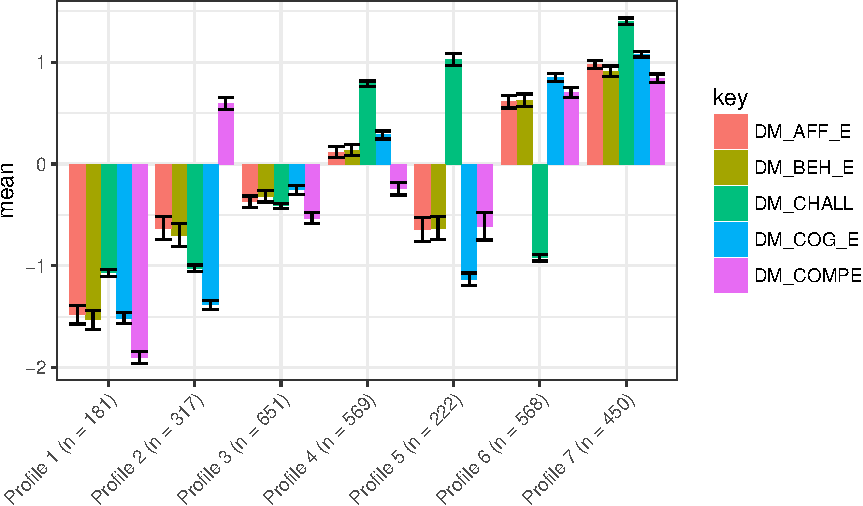
\includegraphics[width=0.9\linewidth]{rosenberg-dissertation_files/figure-latex/m1_7p-1} \end{center}

\begin{center}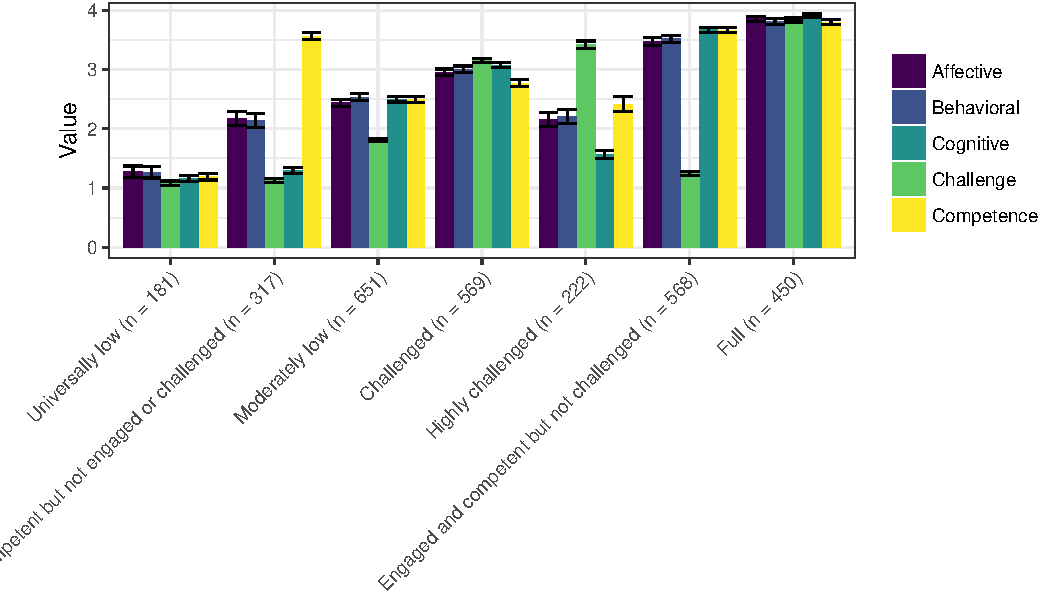
\includegraphics[width=0.9\linewidth]{rosenberg-dissertation_files/figure-latex/m1_7p-2} \end{center}

The number of observations associated with each of the profiles is not
very balanced, with few (\emph{n} = 181) observations associated with
the universally low profile and few (\emph{n} = 222) observations
associated with the highly challenged profile. The number of
observations associated with the other profiles ranged from 317 to 651.
Distinct from other solutions, none of the other five profiles were
found in the other model 1 solutions. Two pairs of the
profiles--challenged and highly challenged and universally low and
moderately low--exhibited similar patterns among the variables that were
distinguished by different mean levels. Taken together, this solution
raises questions about whether it may be too complex, possibly
suggesting preference for model one five and six profile solutions.

\bibliography{book.bib,packages.bib}


\end{document}
